%!TEX root = ../rapport.tex

\chapter{Results}
\newcommand{\exampleheight}{2.2in}

The program implemented is able to draw illustrations of reduction graphs with
several different drawing algorithms. This Chapter contains examples of reduction graphs
drawn by the software. 

The graphs were produced ``randomly'', by experimenting with lambda terms and
adjusting them to exhibit (sometimes) interesting behaviour in their reduction
graphs. We found that the best all-round drawing algorithm to use when
experimenting with terms is the Neato algorithm, since it gives nice graphs
most of the time; the others can give very beautiful graphs sometimes, but
often their output is worse than that of Neato.

For each example graph, the caption text contains an explanation of what is
going on. Thus, the contents of this Chapter is solely to be found in the
images and their captions.

\begin{figure}[htbp]
	% #a.(b) (#x.((x x) x) #y.((y y) y))
	\centering
	\subfigure[Drawn with Dot.]{
		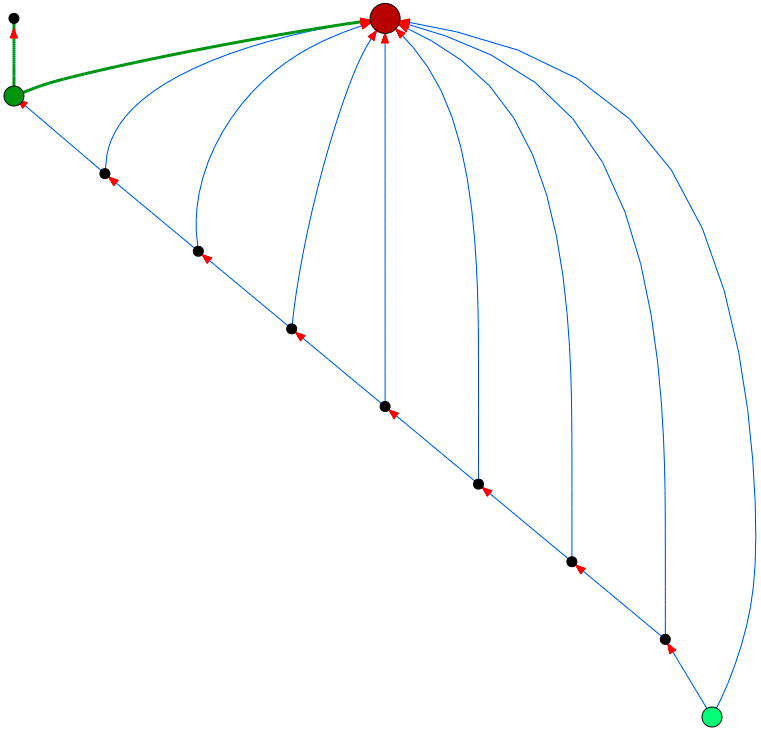
\includegraphics[height=\exampleheight]{../images/inf_reduction_graph_DOT.png}
	}
	\subfigure[Also drawn with Dot, but several generations later.]{
		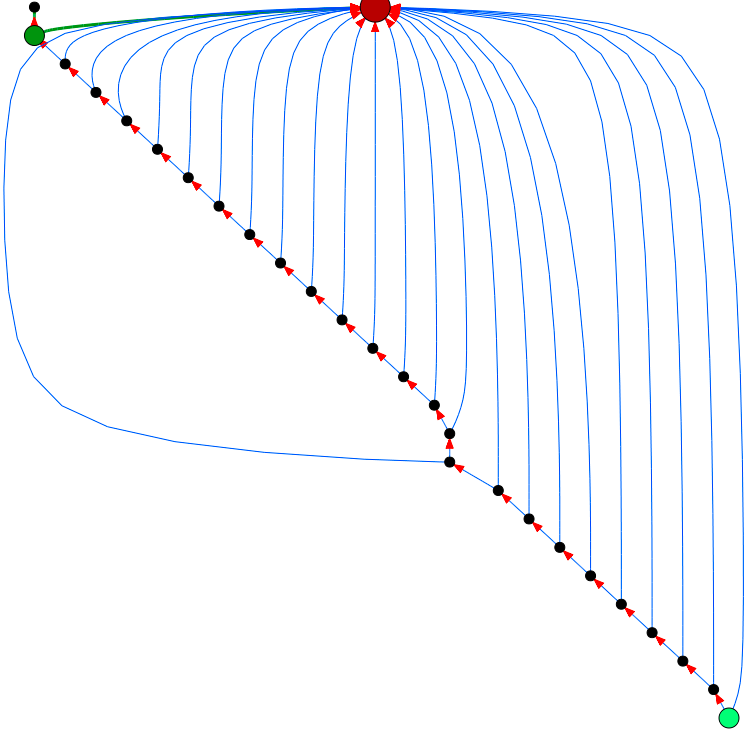
\includegraphics[height=\exampleheight]{../images/inf_reduction_graph_DOT2.png}
	}
	\caption[$(\lam{a}{b}) (\lam{x}{(xxx)} \lam{y}{(yyy)})$]
	{When Dot draws the graph $G_\beta\big((\lam{a}{b}) (\lam{x}{(xxx)} \lam{y}{(yyy)})\big)$
	for later generations, a peculiar phenomenon occurs: one of the nodes on the ``ladder''
	has one of its edges pointing in another way than the equivalent edges of the other
	nodes. This is an artefact of the internal workings of the Dot algorithm.}
	\label{fig:images_inf_reduction_graph_DOT}
\end{figure}

\begin{figure}[htbp]
	% #f.(#x.(f (x x))) (#x.(f (x x))) #y.((y y) y)
	\centering
	\subfigure[Neato.]{
		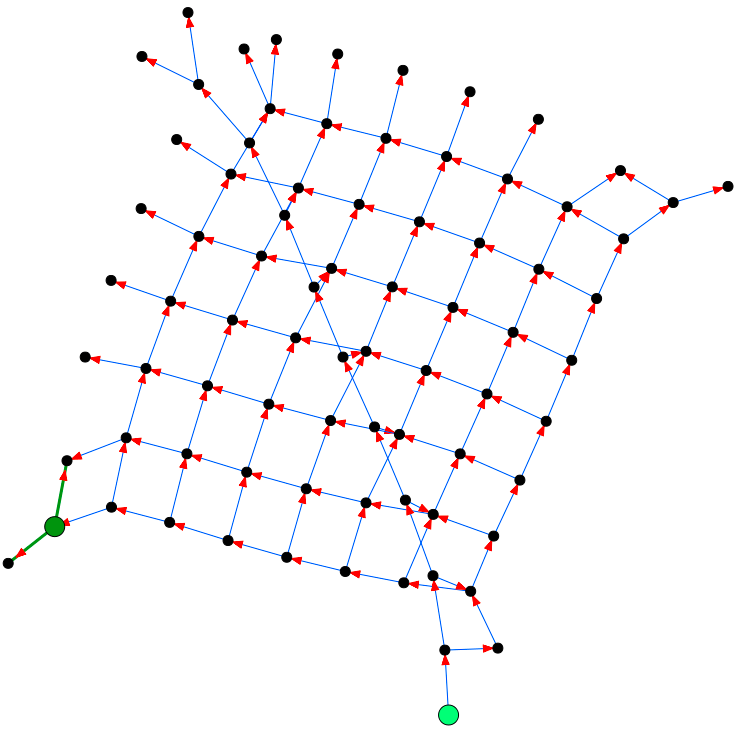
\includegraphics[height=\exampleheight]{../images/Ycomb_1_NEATO.png}
	}
	\subfigure[Twopi.]{
		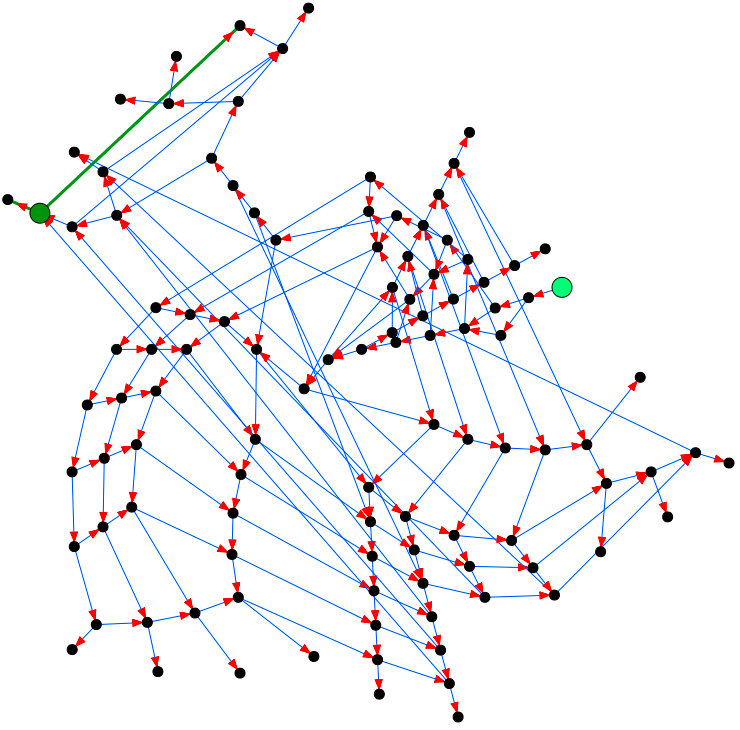
\includegraphics[height=\exampleheight]{../images/Ycomb_1_TWOPI.png}
	}
	\subfigure[Dot.]{
		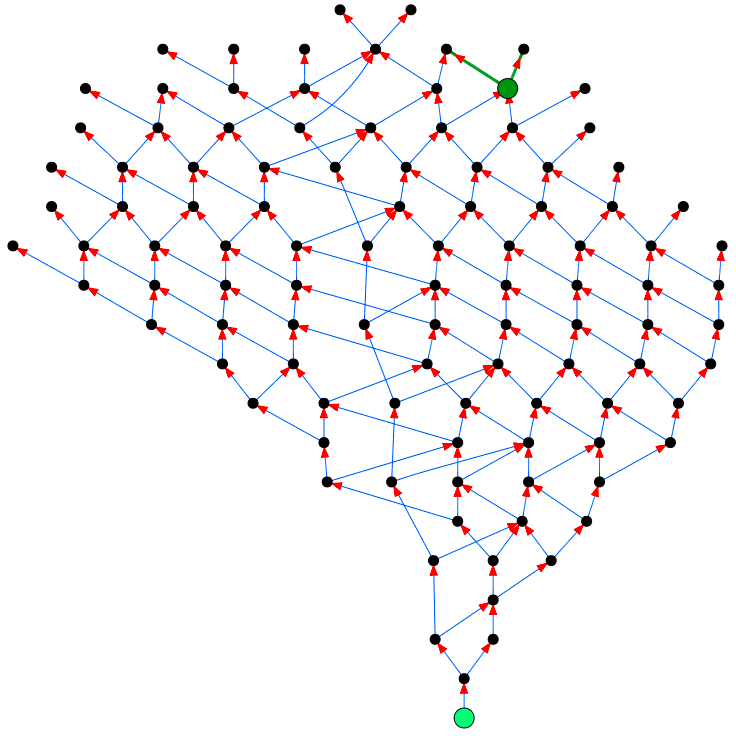
\includegraphics[height=\exampleheight]{../images/Ycomb_1_DOT.png}
	}
	\caption[$(\lam{f}{(\lam{x}{f (x x)}) (\lam{x}{f (x x)})}) \lam{y}{(y y) y}$]
	{The Y-combinator applied to $\omega_3$: $G_\beta\big((\lam{f}{(\lam{x}{f (x x)}) (\lam{x}{f (x x)})}) \lam{y}{(y y) y}\big)$.}
	\label{fig:images_YComb_1}
\end{figure}

\begin{figure}[htbp]
	% ((#b1.(b1) #b2.((#b3.(b2) #b4.((#b5.(b2) b4))))) #b6.((#b7.(b6) #b8.(#b9.(#b10.(#b11.(b11)))))))
	\centering
	\subfigure[Neato]{
		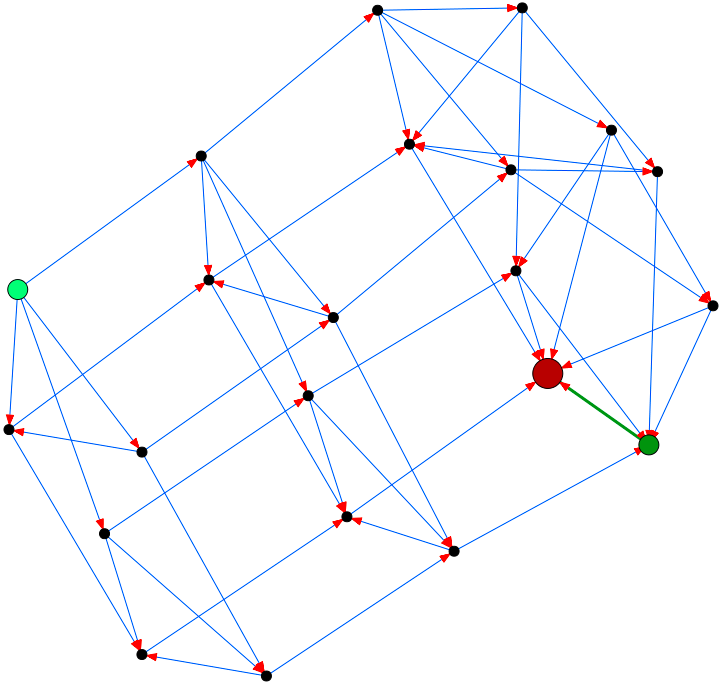
\includegraphics[height=\exampleheight]{../images/finite_ex_1_NEATO.png}
	}
	\subfigure[Dot]{
		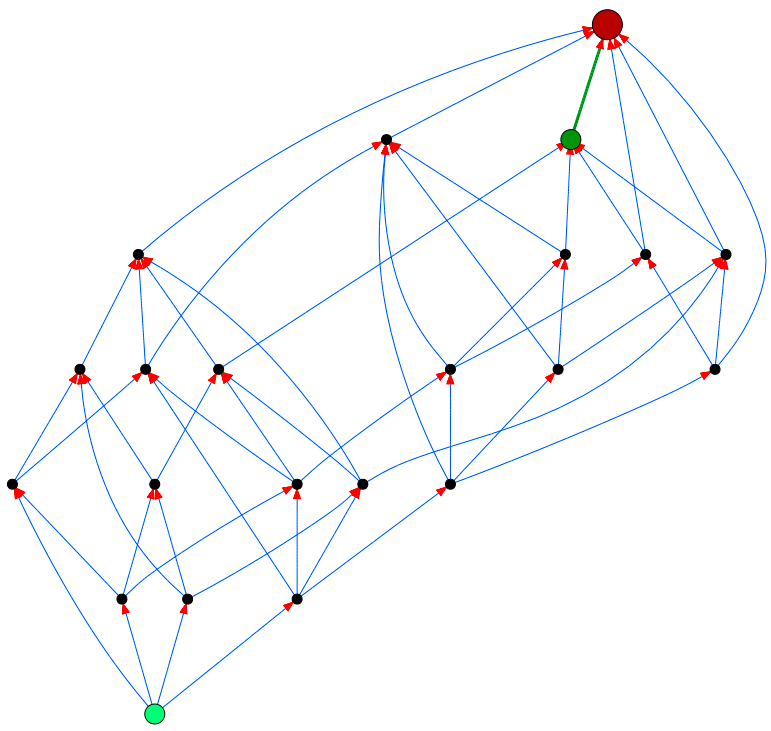
\includegraphics[height=\exampleheight]{../images/finite_ex_1_DOT.png}
	}
	\subfigure[Fdp]{
		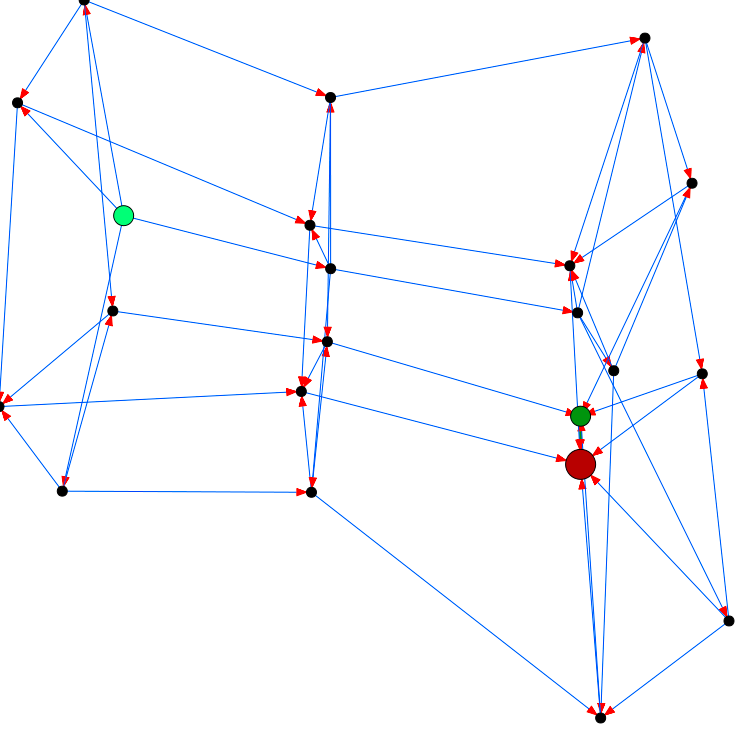
\includegraphics[height=\exampleheight]{../images/finite_ex_1_FDP.png}
	}

	\caption[$((\lam{x}{x}) \lam{y}{((\lam{z}{y}) \lam{z}{((\lam{a}{y}) z)})}) \lam{x}{((\lam{y}{x}) \lam{y}{(\lam{z}{(\lam{a}{\lam{b}{b}})})})}$]
	{This randomly generated lambda term has a box-like embedding of 
	its reduction graph: $G_\beta\big(((\lam{x}{x}) \lam{y}{((\lam{z}{y}) \lam{z}{((\lam{a}{y}) z)})}) \lam{x}{((\lam{y}{x}) \lam{y}{(\lam{z}{(\lam{a}{\lam{b}{b}})})})}\big)$.
	}
	\label{fig:images_finite_ex_1_NEATO}
\end{figure}

\begin{figure}[htbp]
	% (#B1.(#B2.(((#B3.(#B4.(#B5.(#B6.(B1)))) #B7.(#B8.(B7))) (#B9.(B1) #B10.(#B11.(B1)))))) (#B12.(#B13.(B13)) #B14.(#B15.(#B16.((#B17.(B17) B16))))))
	\renewcommand{\exampleheight}{2.5in}
	\centering
	\subfigure[Twopi]{
		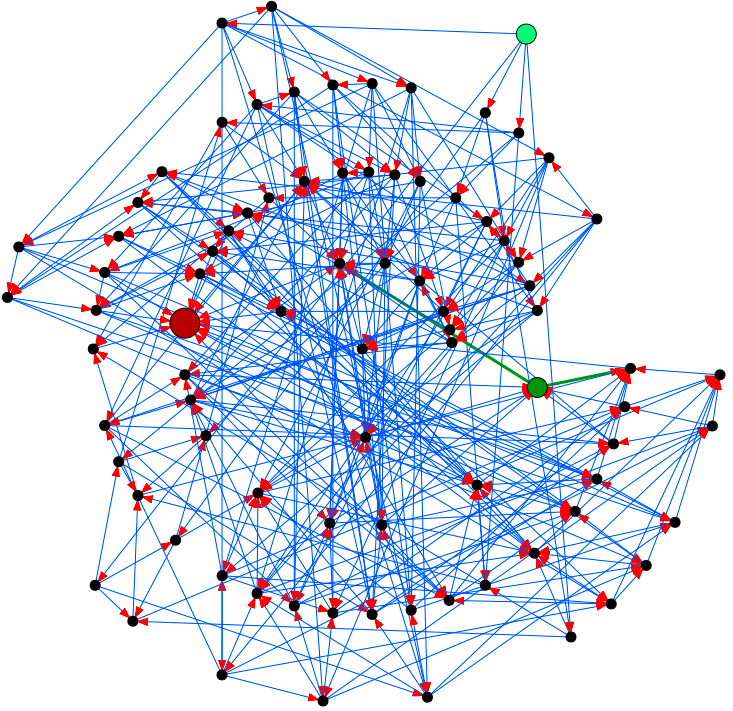
\includegraphics[height=\exampleheight]{../images/finite_ex_2_TWOPI.png}
	}
	\subfigure[Circo]{
		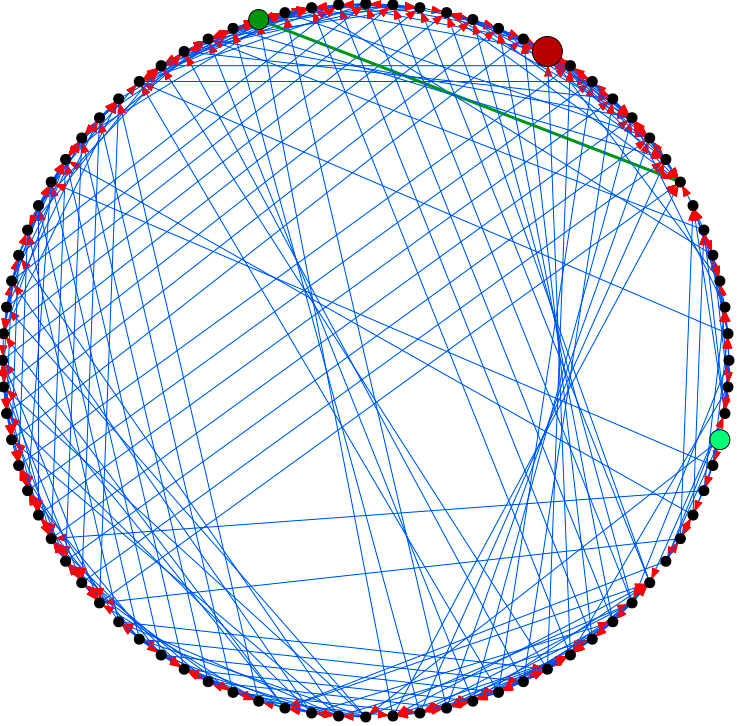
\includegraphics[height=\exampleheight]{../images/finite_ex_2_CIRCO.png}
	}
	\subfigure[Dot]{
		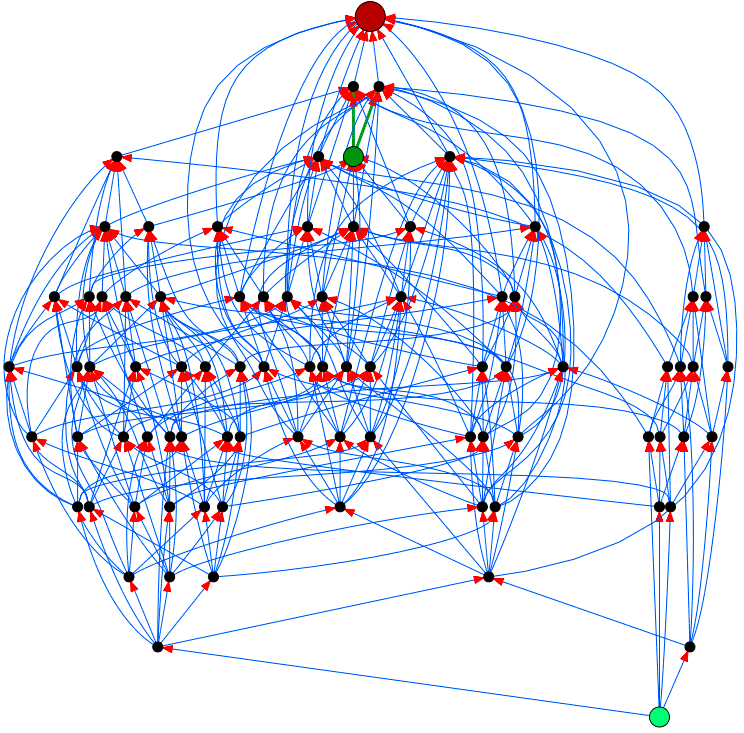
\includegraphics[height=\exampleheight]{../images/finite_ex_2_DOT.png}
	}
	\subfigure[Fdp]{
		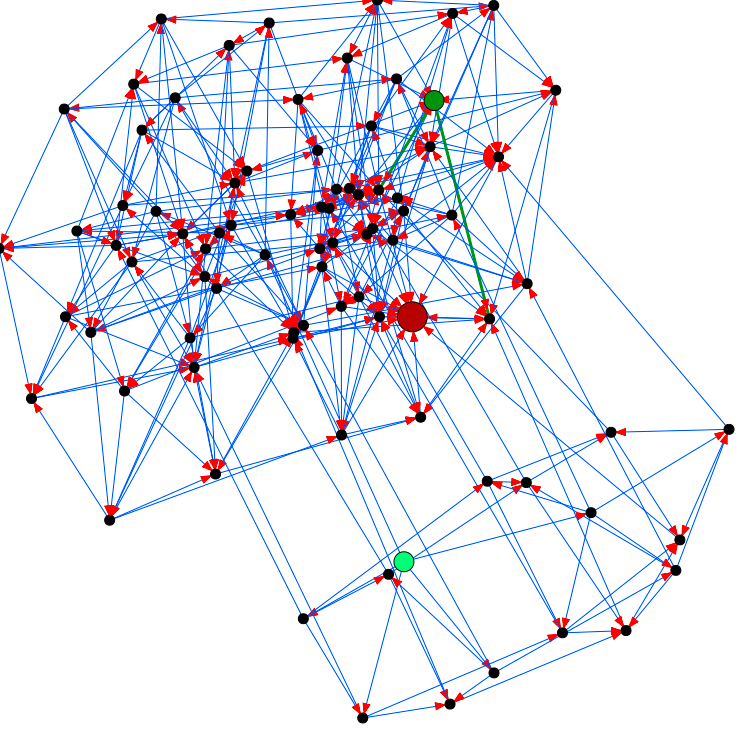
\includegraphics[height=\exampleheight]{../images/finite_ex_2_FDP.png}
	}
	\subfigure[Neato]{
		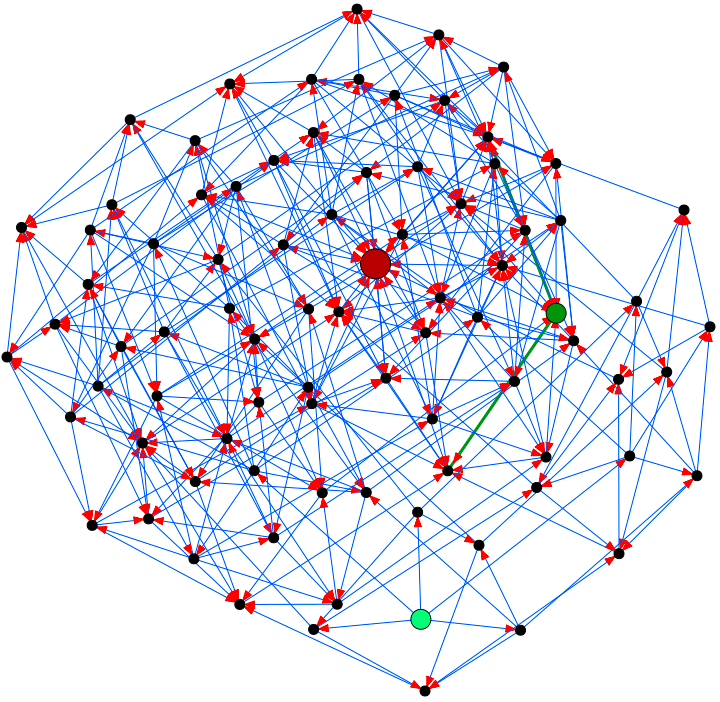
\includegraphics[height=\exampleheight]{../images/finite_ex_2_NEATO.png}
	}
	\subfigure[Majorization]{
		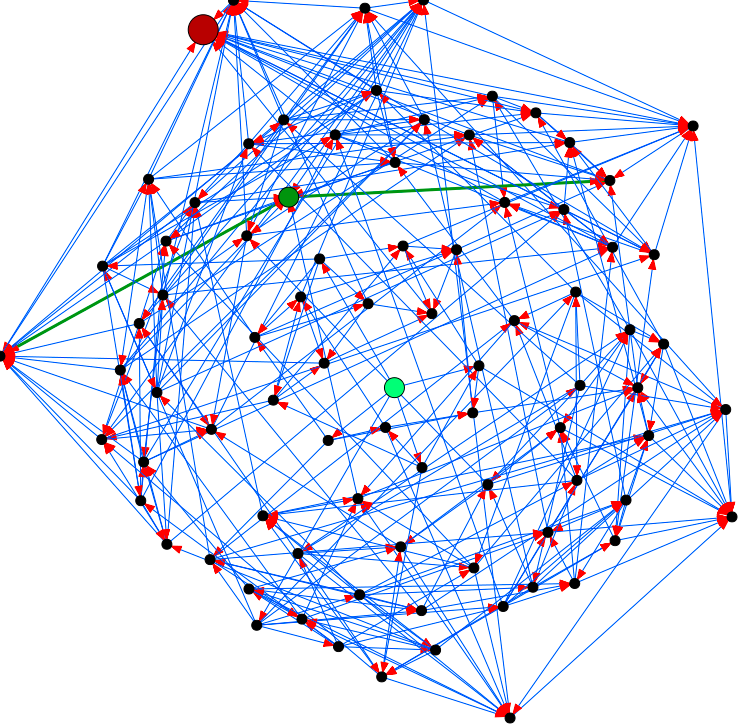
\includegraphics[height=\exampleheight]{../images/finite_ex_2_MAJOR.png}
	}
	
	\caption
	[$\lambda x.(\lambda y.((\lambda z.(\lambda a.(\lambda b.(\lambda c.x))) \lambda z.(\lambda a.z)) (\lambda y.x \lambda z.(\lambda a.x))
	)) (\lambda x.(\lambda y.y) \lambda x.(\lambda y.(\lambda z.(\lambda a.(a) z))))$]
	{Another randomly generated lambda term. In its reduction graph we
	get a clear impression of the differences between the provided drawing algorithms.
	$G_\beta\big(
	\lambda x.(\lambda y.((\lambda z.(\lambda a.(\lambda b.(\lambda c.x))) \lambda z.(\lambda a.z)) (\lambda y.x \lambda z.(\lambda a.x))
	)) (\lambda x.(\lambda y.y) \lambda x.(\lambda y.(\lambda z.(\lambda a.(a) z))))
	\big)$.}
	\label{fig:images_finite_ex_2_CIRCO}
\end{figure}

\begin{figure}[htbp]
	% λB1.((λB2.(λB3.((λB4.((B4 (λB5.(B1) λB6.(λB7.(B7))))) λB8.(B8)))) B1))
	\centering
	\subfigure[Majorization]{
		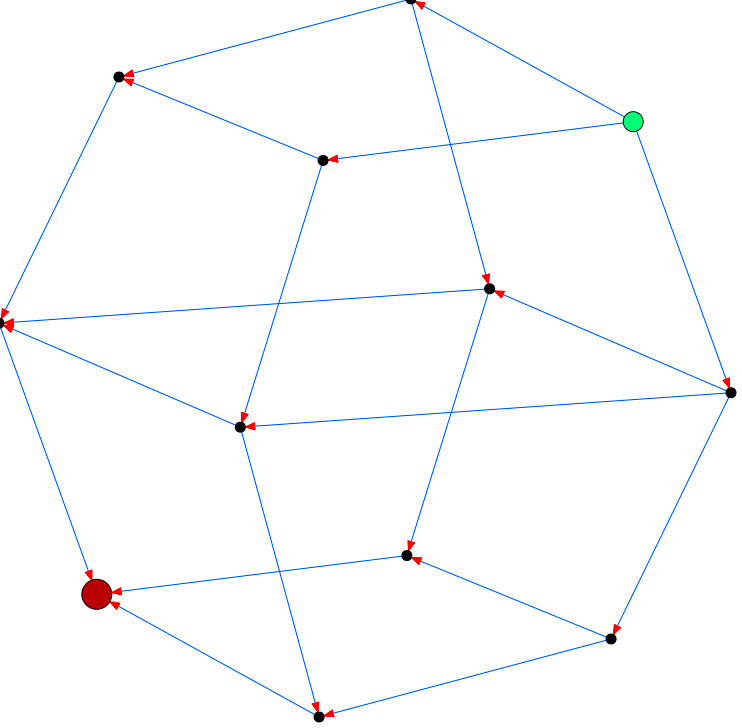
\includegraphics[height=\exampleheight]{../images/finite_ex_3_MAJOR.png}
	}
	\subfigure[Neato]{
		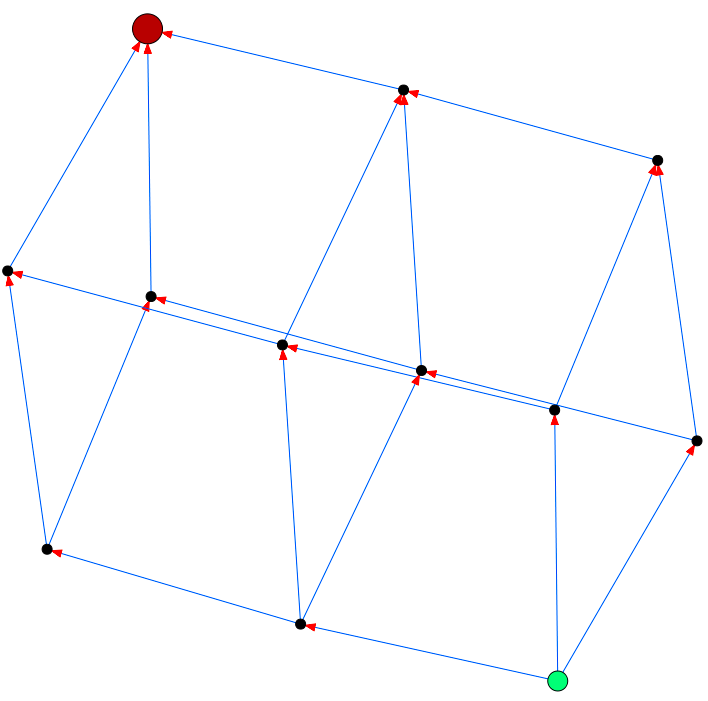
\includegraphics[height=\exampleheight]{../images/finite_ex_3_NEATO.png}
	}
	
	\caption
	[$\lambda x.(\lambda y.(\lambda z.(\lambda a.(a ((\lambda b.x) (\lambda c.\lambda d.d))) \lambda e.e)) x)$]
	{The two force-directed algorithms, Neato and Majorization, differ
	only on subtleties. $G_\beta\big(\lambda x.(\lambda y.(\lambda z.(\lambda a.(a ((\lambda b.x) (\lambda c.\lambda d.d))) \lambda e.e)) x)\big)$.}
	\label{fig:images_finite_ex_3_MAJOR}
\end{figure}

\begin{figure}[htbp]
	% #f.(#x.(f (x x))) (#x.(f (x x))) #y.(y y)
	\centering
	\subfigure[Circo]{
		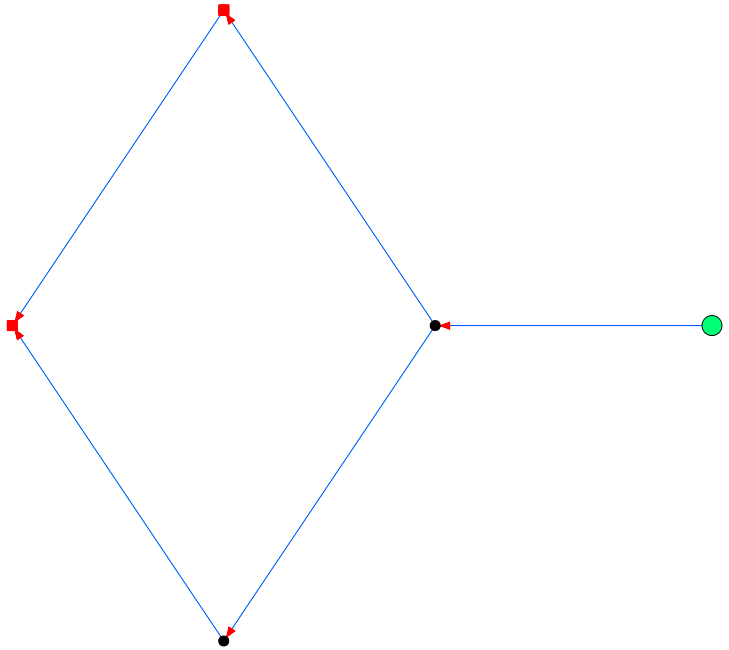
\includegraphics[height=\exampleheight]{../images/Ycomb_2_CIRCO.png}
	}
	\subfigure[Majorization]{
		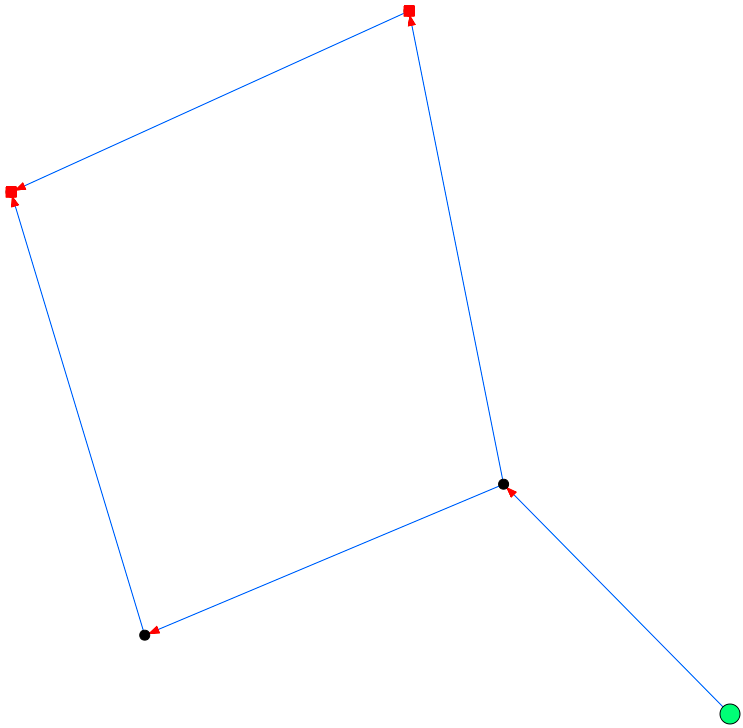
\includegraphics[height=\exampleheight]{../images/Ycomb_2_MAJOR.png}
	}
	
	\caption
	[$\lambda f.(\lambda x.(f (x x))) (\lambda x.(f (x x))) \lambda y.(y y)$]
	{The Y-combinator applied to $\omega$: $\lambda f.(\lambda x.(f (x x))) (\lambda x.(f (x x))) \lambda y.(y y)$.
	No normal form exists, but there is a node from which the reduction operation
	cannot ``escape'' when it is first met.}
	\label{fig:images_Ycomb_2_CIRCO}
\end{figure}
\begin{figure}[htbp]
	% #f.(#x.(f (x x))) (#x.(f (x x))) #x.#y.(y y x)
	\centering
	\subfigure[Majorization]{
		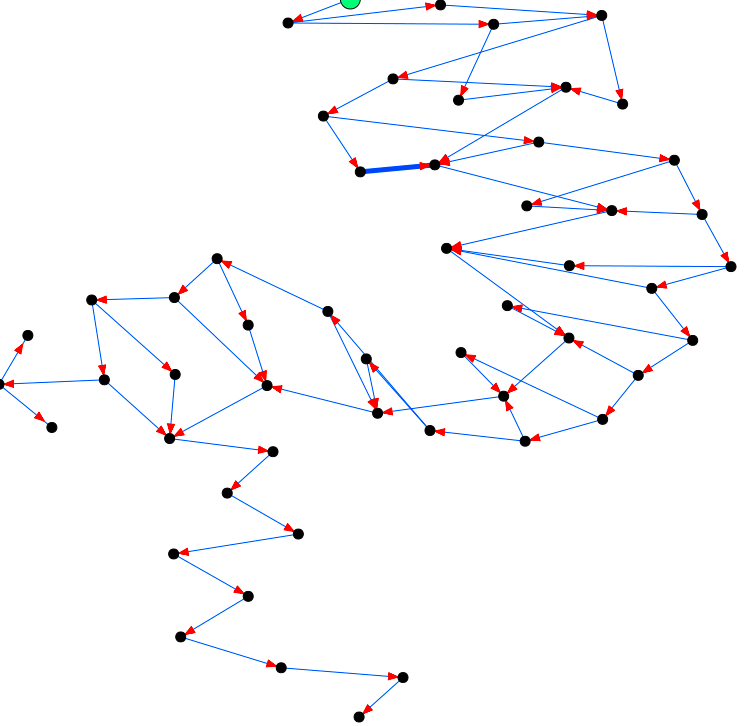
\includegraphics[height=\exampleheight]{../images/Ycomb_3_MAJOR.png}
	}
	\subfigure[Majorization, after more generations.]{
		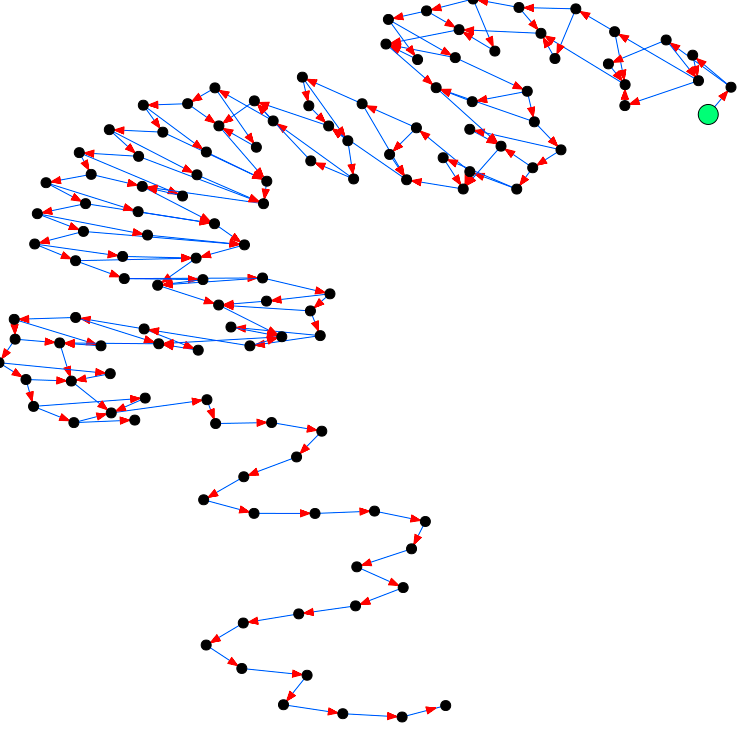
\includegraphics[height=\exampleheight]{../images/Ycomb_3_MAJOR2.png}
	}
	\subfigure[Neato]{
		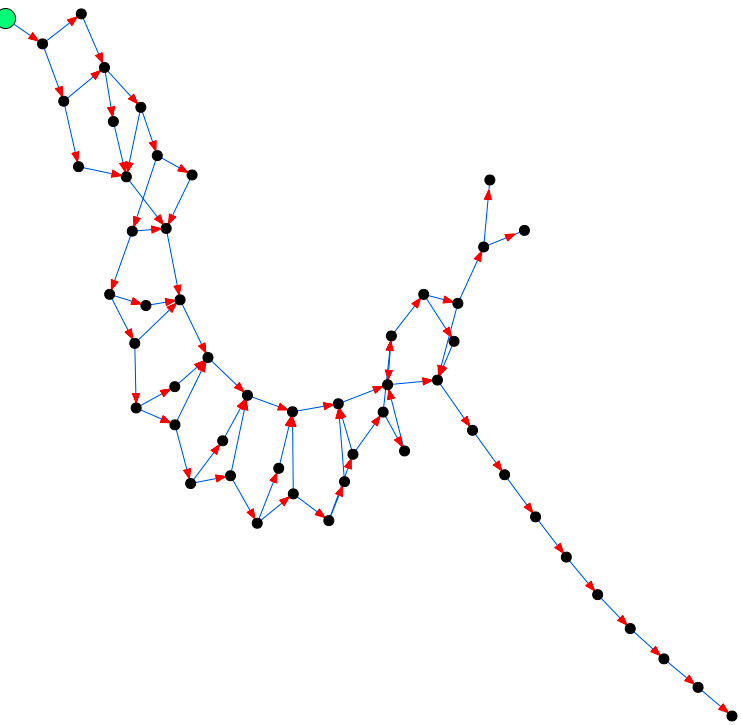
\includegraphics[height=\exampleheight]{../images/Ycomb_3_NEATO.png}
	}
	\subfigure[Neato, after more generations.]{
		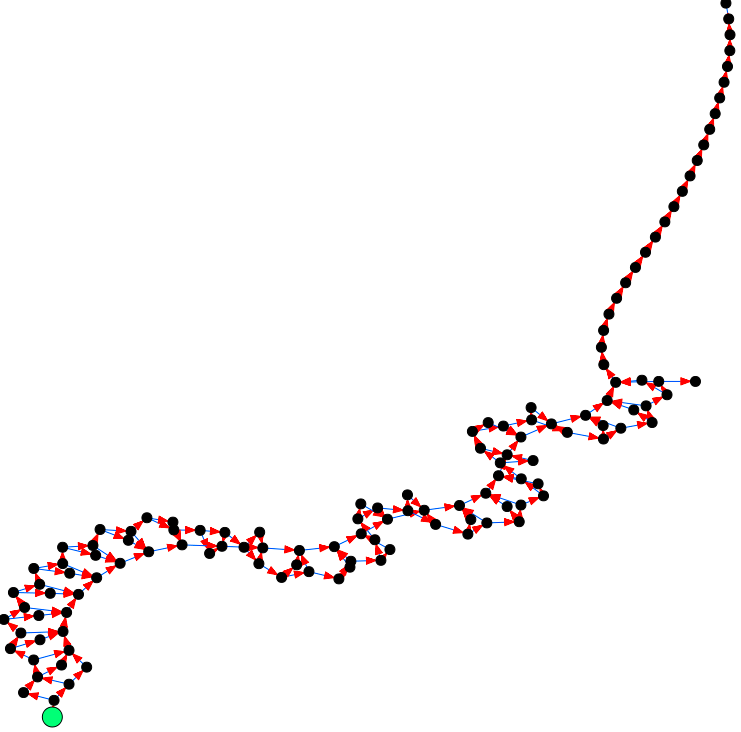
\includegraphics[height=\exampleheight]{../images/Ycomb_3_NEATO2.png}
	}
	\subfigure[Circo]{
		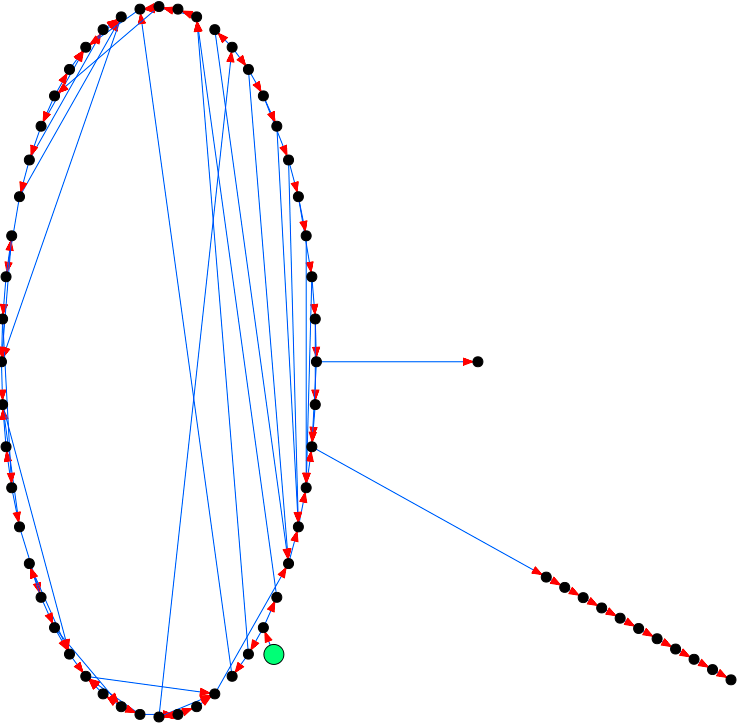
\includegraphics[height=\exampleheight]{../images/Ycomb_3_CIRCO.png}
	}
	\subfigure[Circo one step further; the lone outlier node emits new pairs of nodes.]{
		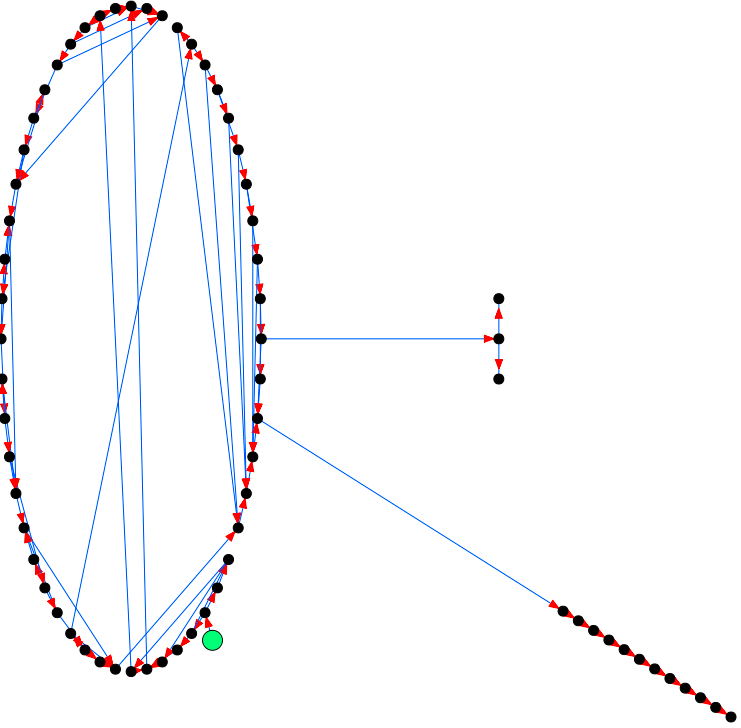
\includegraphics[height=\exampleheight]{../images/Ycomb_3_CIRCO2.png}
	}
	
	\caption
	[$\lambda f.\lambda x.(f (x x)) (\lambda x.f (x x)) \lambda x.\lambda y.(y y x)$]
	{The Y-combinator applied to $\lambda x.\lambda y.(y y x)$: $\lambda f.\lambda x.(f (x x)) (\lambda x.f (x x)) \lambda x.\lambda y.(y y x)$.
	This graph has an interesting property in that it appears to have two ``modes'';
	one where the ``path'' is thick, or broad, and one where we see a simple line
	of nodes next to each other. In some of the graph embeddings the first part
	looks almost like a helix.}
	\label{fig:images_Ycomb_3_1}
\end{figure}

\begin{figure}[htbp]
	% #f.(#x.(f (x x))) (#x.(f (x x))) #x.#y.(y y x)
	\centering
	\subfigure[Dot]{
		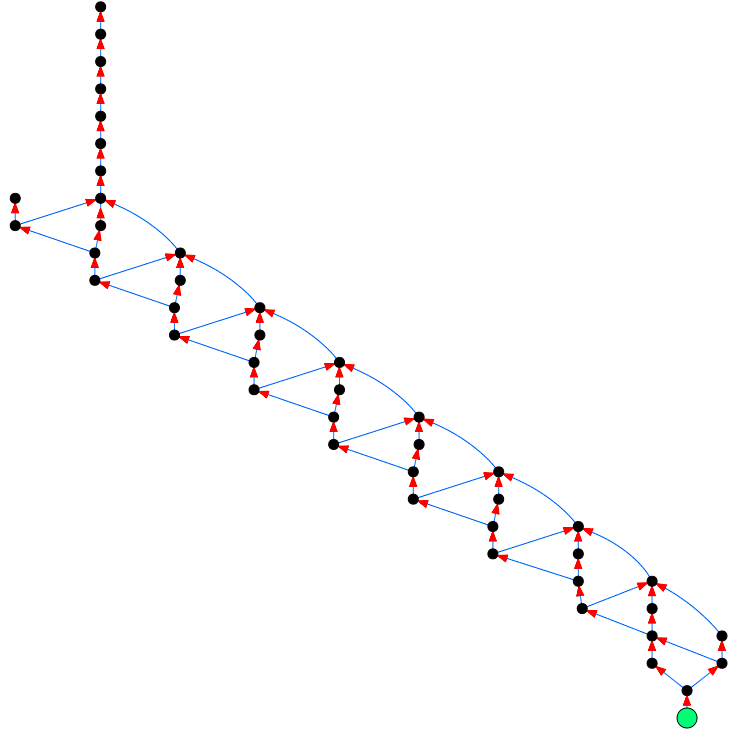
\includegraphics[height=\exampleheight]{../images/Ycomb_3_DOT.png}
	}
	\subfigure[Dot, after more generations.]{
		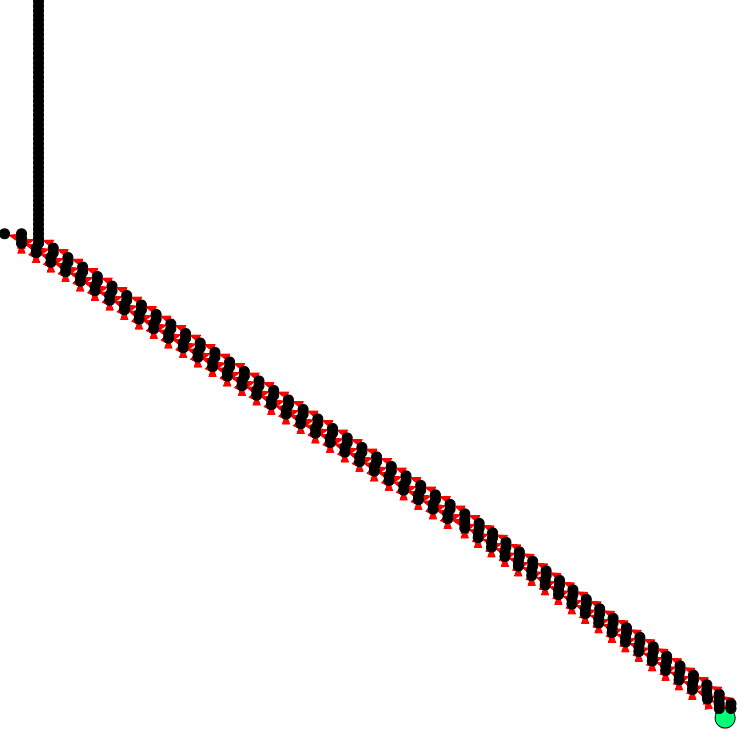
\includegraphics[height=\exampleheight]{../images/Ycomb_3_DOT2.png}
	}
	\subfigure[Fdp]{
		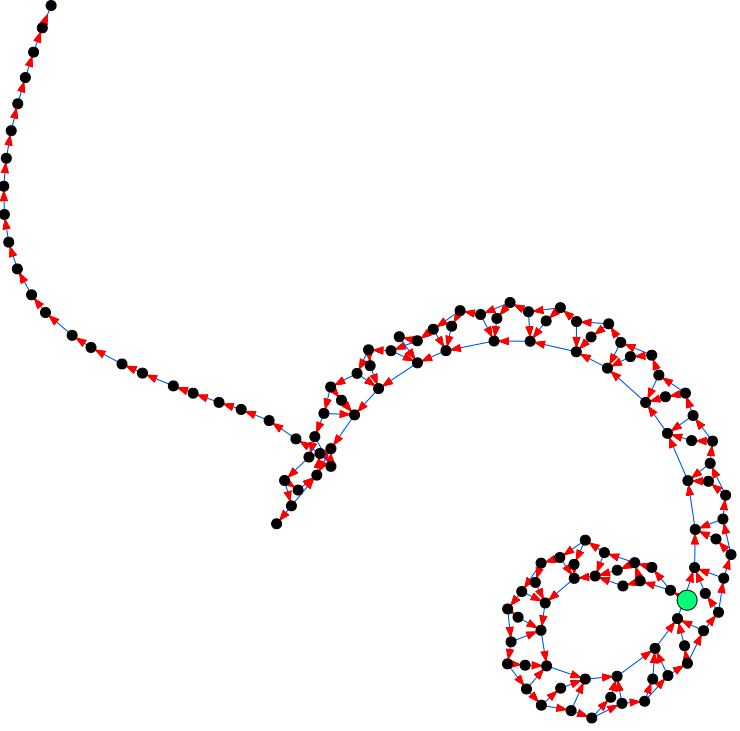
\includegraphics[height=\exampleheight]{../images/Ycomb_3_FDP.png}
	}
	\subfigure[Fdp, after more generations.]{
		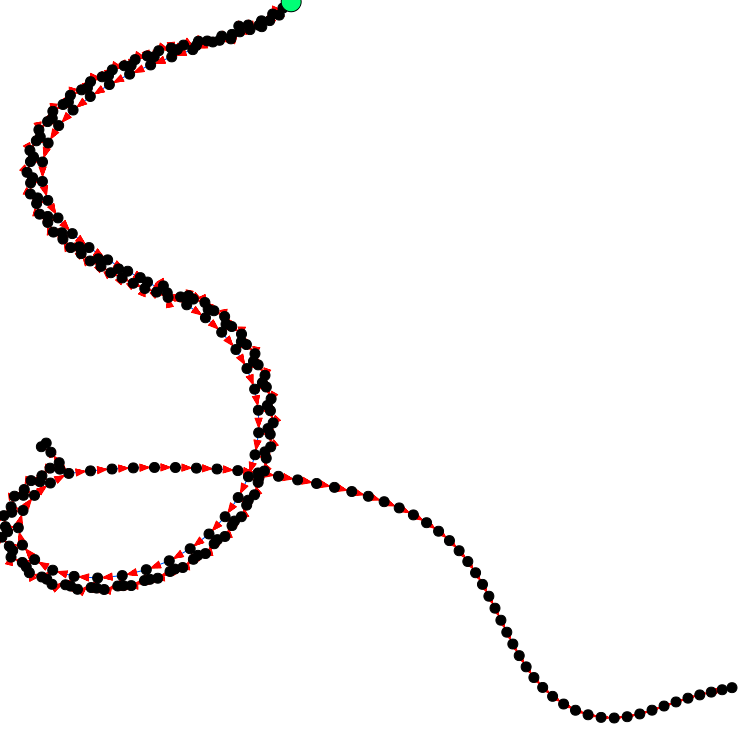
\includegraphics[height=\exampleheight]{../images/Ycomb_3_FDP2.png}
	}
	\subfigure[Twopi]{
		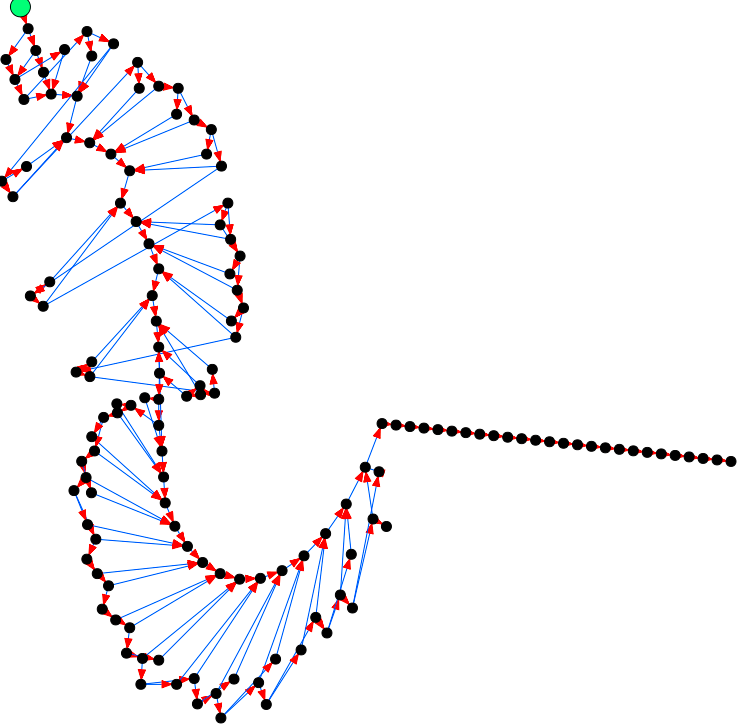
\includegraphics[height=\exampleheight]{../images/Ycomb_3_TWOPI.png}
	}
	\subfigure[Twopi, after more generations.]{
		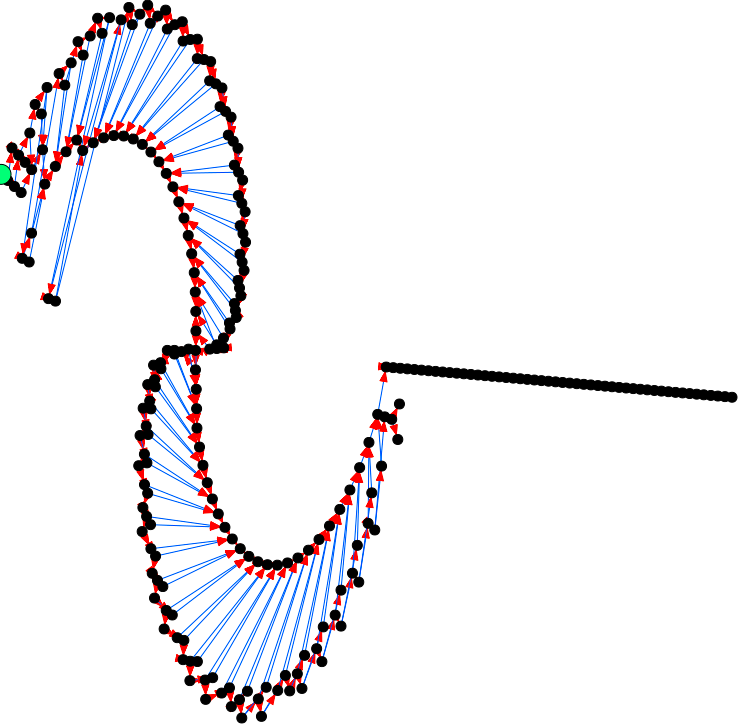
\includegraphics[height=\exampleheight]{../images/Ycomb_3_TWOPI2.png}
	}
	\caption
	[$\lambda f.\lambda x.(f (x x)) (\lambda x.f (x x)) \lambda x.\lambda y.(y y x)$]
	{The same lambda term as in Figure \ref{fig:images_Ycomb_3_1}.}
	\label{fig:images_Ycomb_3_2}
\end{figure}


\begin{figure}[htbp]
	% #x.(#y.(#x.(#y.(#s.(s x y))) #x.(#y.y) (#x.(#y.(#s.(s x y))) x y))) #f.(#x.(f (f x))) #f.(#x.(f (f (f x))))
	% cons(2,3)
	\centering
	\subfigure[$cons(2,3)$: ]{
		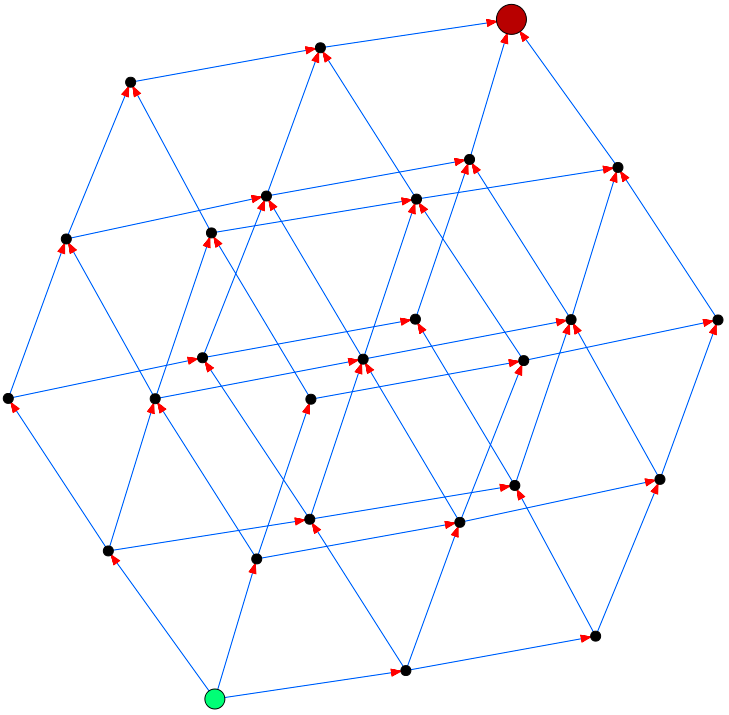
\includegraphics[height=\exampleheight]{../images/Cons23_NEATO.png}
	}
	\subfigure[$cons(5,0)$: ]{
		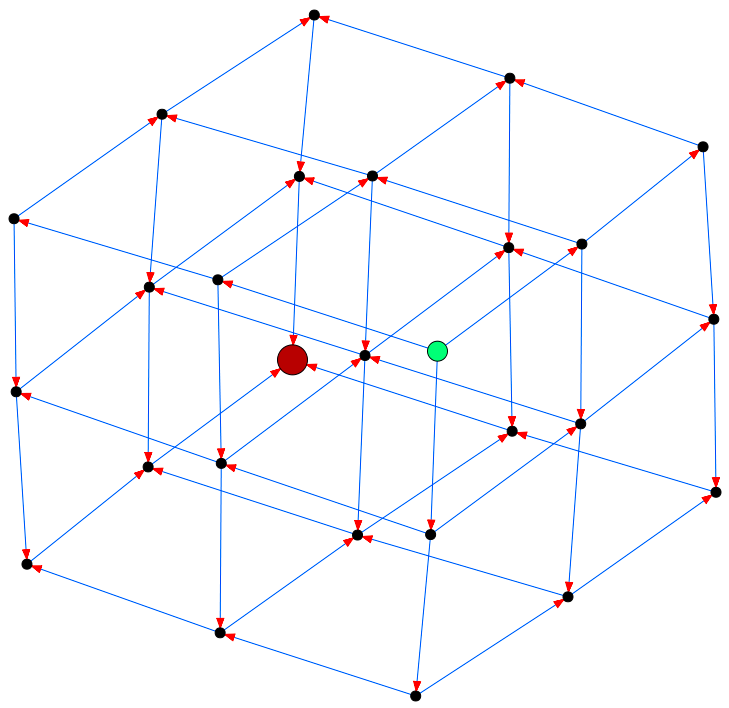
\includegraphics[height=\exampleheight]{../images/Cons50_NEATO.png}
	}
	\subfigure[$cons(4,4)$: ]{
		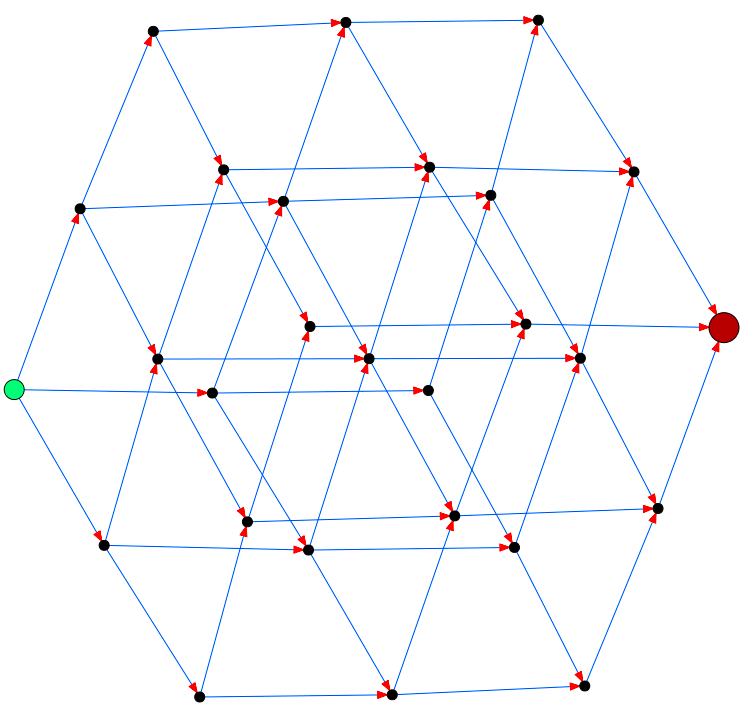
\includegraphics[height=\exampleheight]{../images/Cons44_NEATO.png}
	}
	\begin{tabular}{ll}
		$cons(2,3)$	& $\lambda x.(\lambda y.(\lambda x.(\lambda y.(\lambda s.(s x y))) \lambda x.(\lambda y.y) (\lambda x.(\lambda y.(\lambda s.(s x y))) x y))) \lambda f.(\lambda x.(f (f x))) \lambda f.(\lambda x.(f (f (f x))))$ \\
		$cons(5,0)$ & $\lambda x.(\lambda y.(\lambda x.(\lambda y.(\lambda s.(s x y))) \lambda x.(\lambda y.y) (\lambda x.(\lambda y.(\lambda s.(s x y))) x y))) \lambda f.(\lambda x.(f (f (f (f x))))) \lambda f.(\lambda x.(x))$ \\
		$cons(4,4)$ & $\lambda x.(\lambda y.(\lambda x.(\lambda y.(\lambda s.(s x y))) \lambda x.(\lambda y.y) (\lambda x.(\lambda y.(\lambda s.(s x y))) x y))) \lambda f.(\lambda x.(f (f (f x)))) \lambda f.(\lambda x.(f (f (f x))))$
	\end{tabular}
	\caption
	[The ``cons'' function applied to Church numerals.]
	{The ``cons'' function applied to different Church numerals appears to have
	the same reduction graph. Drawn with Neato.}
	\label{fig:images_Cons_NEATO}
\end{figure}

\begin{figure}[htbp]
	\centering
	% #n.(#f.(#x.(f (n f x)))) #f.(#x.(f (f (f (f (f x))))))
	\subfigure[Successor to 5.]{
		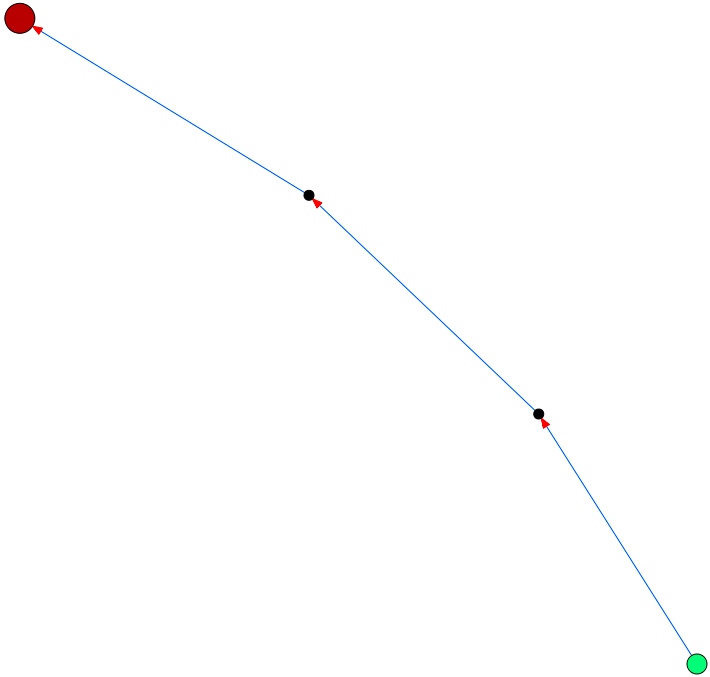
\includegraphics[height=\exampleheight]{../images/Succ5_NEATO.png}
	}
	% #n.(#f.(#x.(n (#g.(#h.(h (g f)))) (#u.(x)) (#u.(u))))) #f.(#x.(f (f (f (f (f x))))))
	\subfigure[Predecessor to 5.]{
		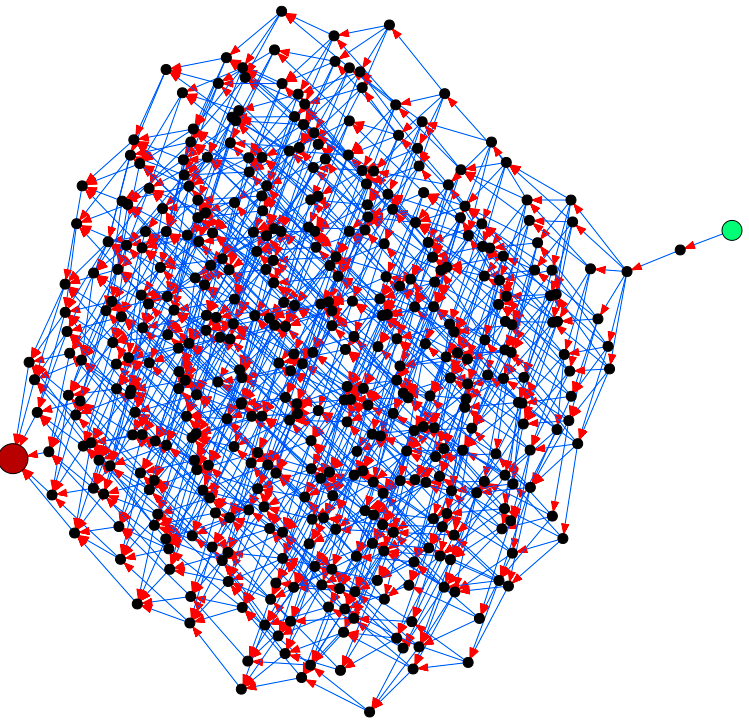
\includegraphics[height=\exampleheight]{../images/Pred5_NEATO.png}
	}
	\begin{tabular}{ll}
		$succ(5)$ & $\lambda n.(\lambda f.(\lambda x.(f (n f x)))) \lambda f.(\lambda x.(f (f (f (f (f x))))))$ \\
		$pred(5)$ & $\lambda n.(\lambda f.(\lambda x.(n (\lambda g.(\lambda h.(h (g f)))) (\lambda u.(x)) (\lambda u.(u))))) \lambda f.(\lambda x.(f (f (f (f (f x))))))$
	\end{tabular}
	
	\caption[The successor and predecessor function.]
	{Neato drawings of the successor and predecessor functions applied
	to the Church numeral for five. The story goes that the predecessor function 
	was though up by Kleene while at the dentist, where he was anaesthesized by laughing gas. 
	The reduction graph of the function somehow confirms this story.}
	\label{fig:images_Succ5_NEATO}
\end{figure}


\begin{figure}[htbp]
	\centering

	% #m.(#n.(#f.(#x.(m f (n f x))))) #f.(#x.(f (f x))) #f.(#x.(f (f x)))
	\subfigure[$2+2$]{
		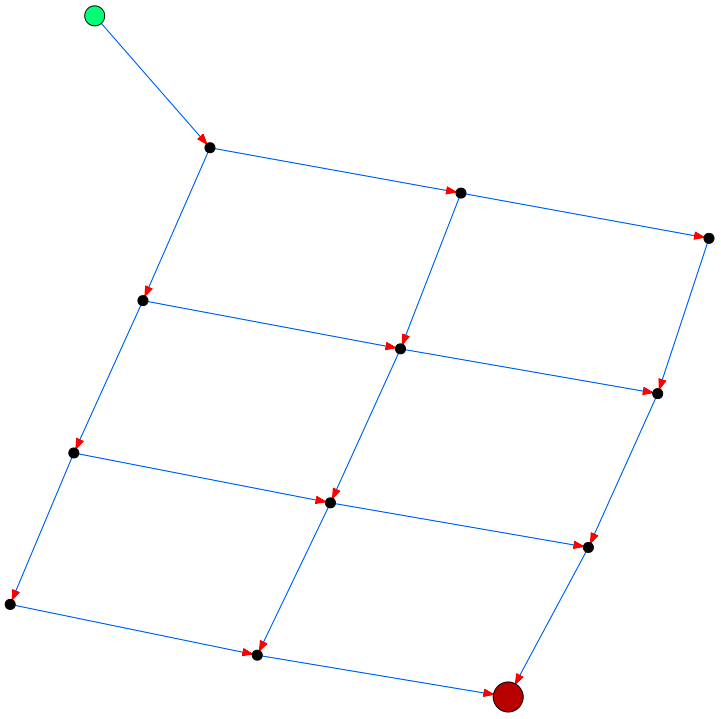
\includegraphics[height=\exampleheight]{../images/Sum22_NEATO.png}
	}
	% #m.(#n.(#f.(#x.(m (n f) x)))) #f.(#x.(f (f x))) #f.(#x.(f (f x)))
	\subfigure[$2\cdot 2$]{
		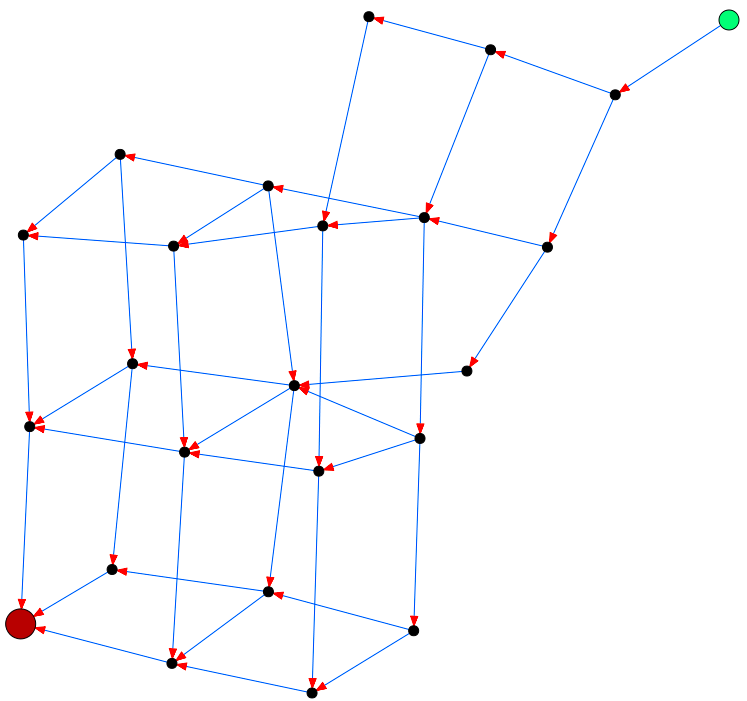
\includegraphics[height=\exampleheight]{../images/Prod22_NEATO.png}
	}
	% #m.(#n.(#f.(#x.(m n f x)))) #f.(#x.(f (f x))) #f.(#x.(f (f x)))
	\subfigure[$2^2$]{
		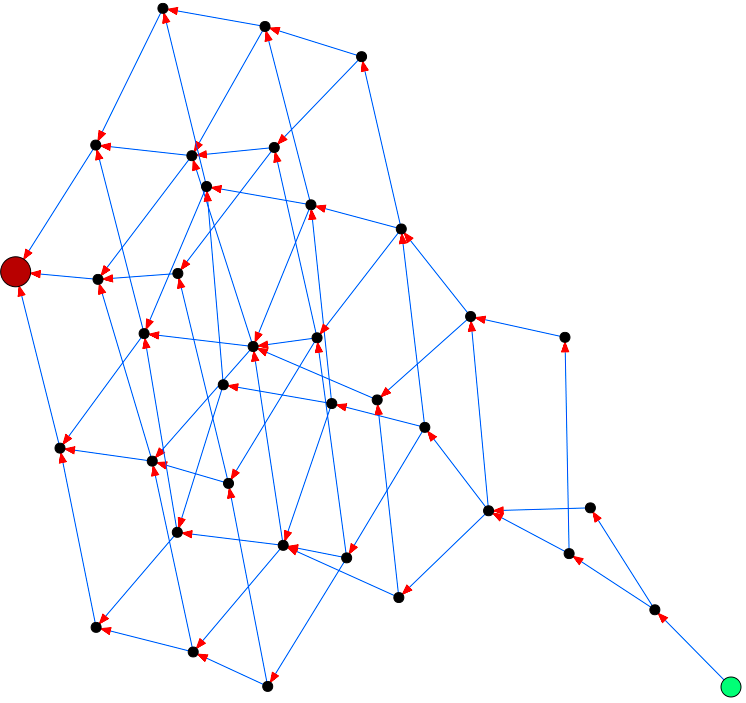
\includegraphics[height=\exampleheight]{../images/Exp22_NEATO.png}
	}
	\begin{tabular}{ll}
		$2+2$ & $\lambda m.(\lambda n.(\lambda f.(\lambda x.(m f (n f x))))) \lambda f.(\lambda x.(f (f x))) \lambda f.(\lambda x.(f (f x)))$ \\
		$2\cdot 2$ & $\lambda m.(\lambda n.(\lambda f.(\lambda x.(m (n f) x)))) \lambda f.(\lambda x.(f (f x))) \lambda f.(\lambda x.(f (f x)))$ \\
		$2^2$ & $\lambda m.(\lambda n.(\lambda f.(\lambda x.(m n f x)))) \lambda f.(\lambda x.(f (f x))) \lambda f.(\lambda x.(f (f x)))$
	\end{tabular}
	\caption[Addition, multiplication and exponentiation.]
	{Different ways to produce the Church numeral for 4. The reduction
	graphs convey the impression that exponentiation is ``greater than'' multiplication
	which is again ``greater than'' addition, in the sense that exponentiation is repetated multiplication
	and multiplication is repeated addition. The graphs are drawn with the Neato
	algorithm.}
	\label{fig:images_22_NEATO}
\end{figure}

\begin{figure}[htbp]
	%  #x.(x x (x x)) #x.(x x f)
	\centering
	\subfigure[Drawn with Dot.]{
		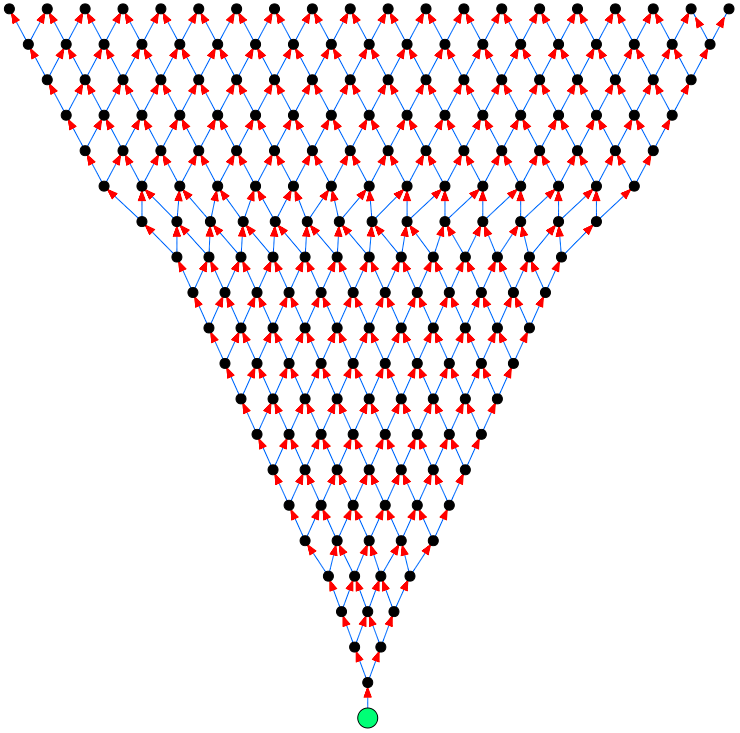
\includegraphics[height=\exampleheight]{../images/grid_1_DOT.png}
	}
	\subfigure[Drawn with Neato.]{
		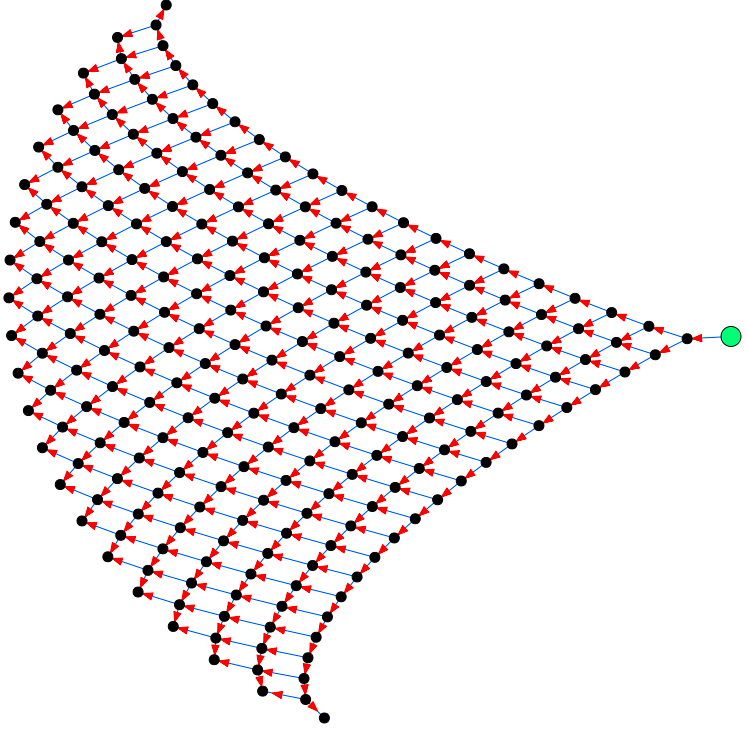
\includegraphics[height=\exampleheight]{../images/grid_1_NEATO.png}
	}
	
	\caption
	[$\lambda x.(x x (x x)) \lambda x.(x x f)$]
	{These drawings of $G_\beta\big(\lambda x.(x x (x x)) \lambda x.(x x f)\big)$ 
	gives rise to comparisons to the Cantor set. Because of the Church-Rosser property,
	no trees can be reduction graphs, so the closest we get to something \emph{resembling}
	the Cantor set is probably something that looks like this.}
	\label{fig:images_grid_1_DOT}
\end{figure}

\begin{figure}[htbp]
	% #x.(x x) #x.(x x) (#x.(x x c) #x.(x x d))
	\centering
		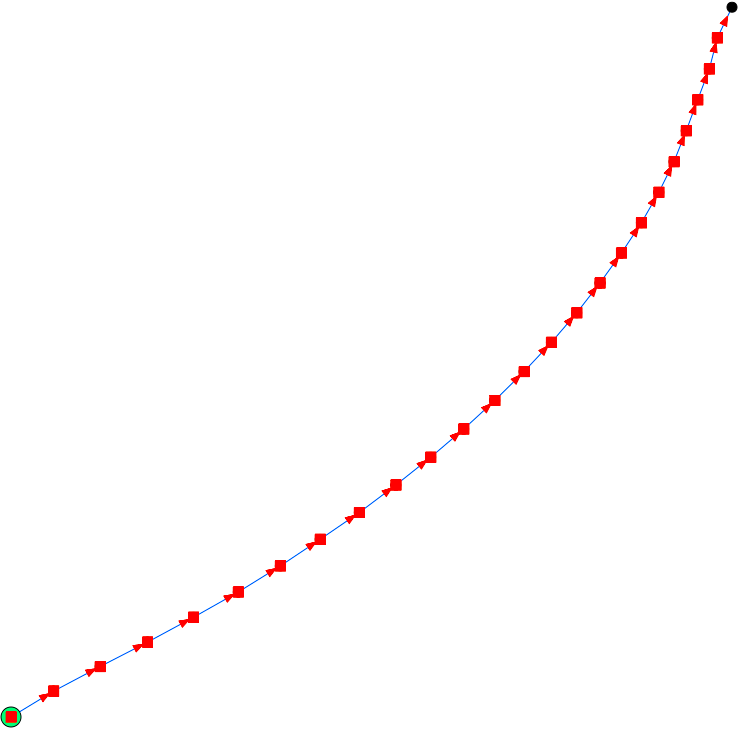
\includegraphics[height=\exampleheight]{../images/Snake_1_NEATO.png}
	\caption[$\lambda x.(x x) \lambda x.(x x) (\lambda x.(x x c) \lambda x.(x x d))$]
	{This alternative version of the ``snake'' has a self-referencing edge
	in every node. The black node at the tip is there because its redexes have not been
	reduced yet, whence the self-referencing edge does not yet exist. The graph is drawn
	with Neato.
	$G_\beta\big(\lambda x.(x x) \lambda x.(x x) (\lambda x.(x x c) \lambda x.(x x d))\big)$.}
	\label{fig:images_Snake_1_NEATO}
\end{figure}

\begin{figure}[htbp]
	% #x.(x a) (#x.(x x b) #x.(x x c))
	\centering
	\subfigure[Circo.]{
		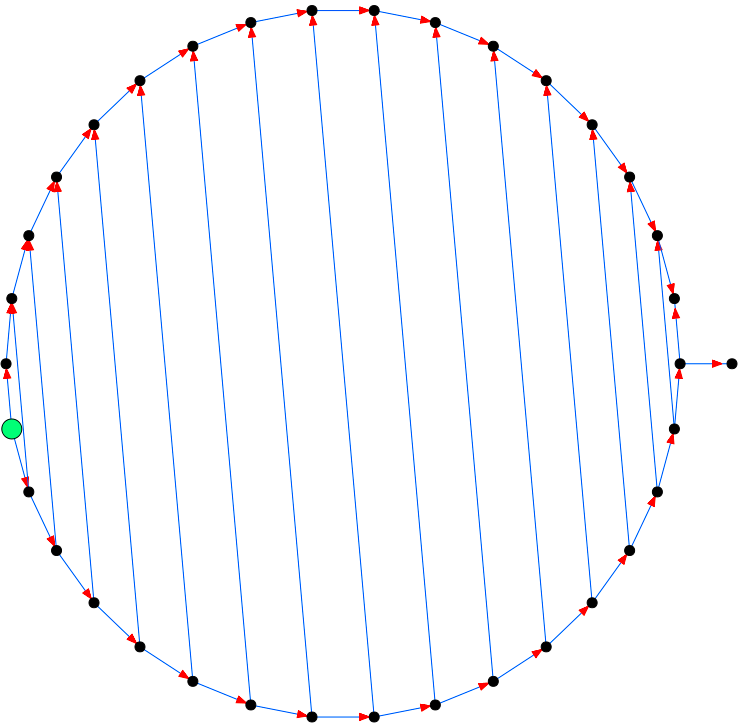
\includegraphics[height=\exampleheight]{../images/DoubleSnake_1_CIRCO.png}
	}
	\subfigure[Dot.]{
		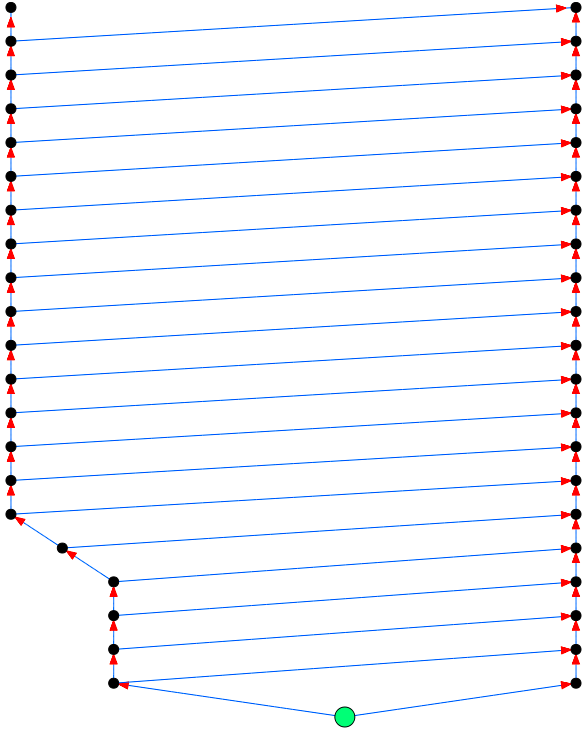
\includegraphics[height=\exampleheight]{../images/DoubleSnake_1_DOT.png}
	}
	\subfigure[Neato.]{
		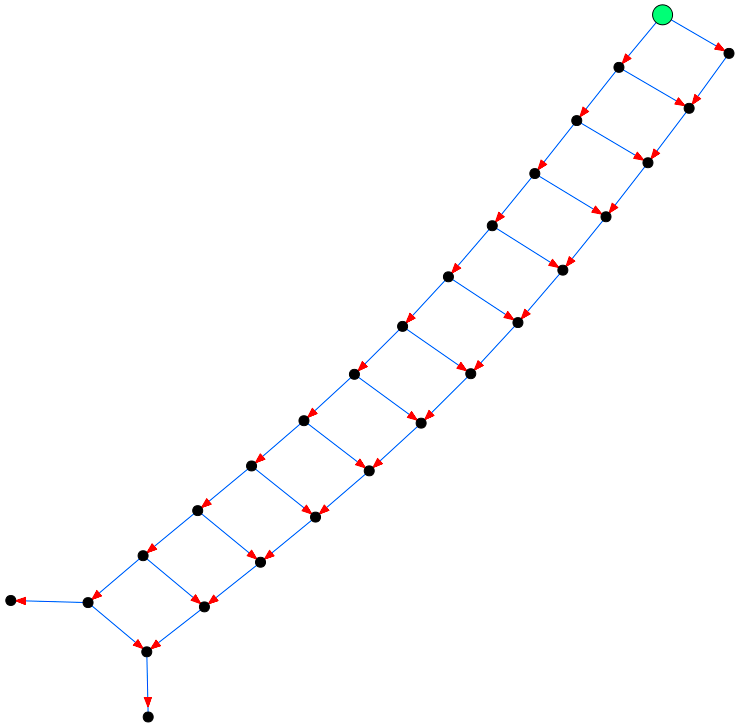
\includegraphics[height=\exampleheight]{../images/DoubleSnake_1_NEATO.png}
	}
	\subfigure[Twopi.]{
		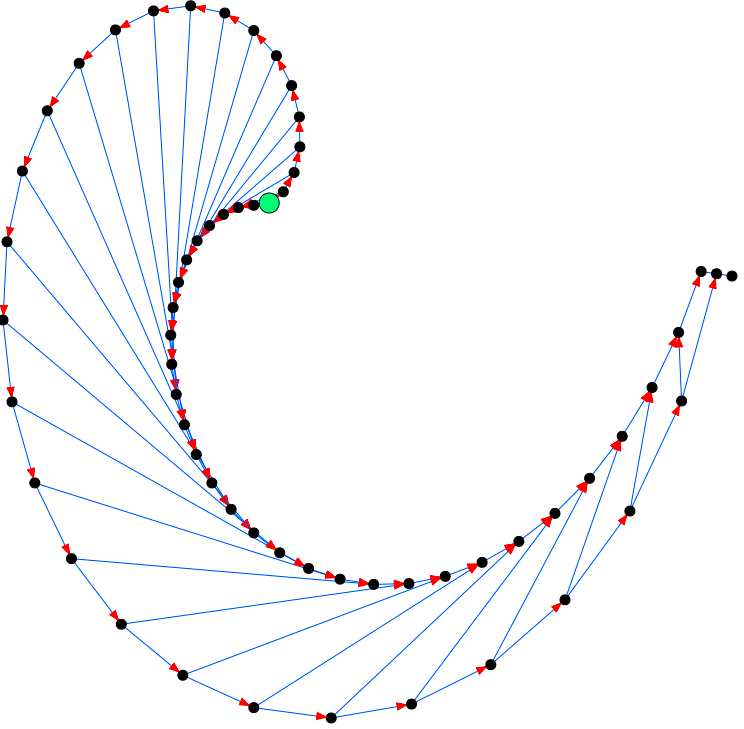
\includegraphics[height=\exampleheight]{../images/DoubleSnake_1_TWOPI.png}
	}

	\caption[$\I(\omega_n \omega_n)$, $n\geq 3$]
	{The graph $G_\beta\big(\I(\omega_n \omega_n)\big)$ for $n\geq 3$ gives
	nice, regular drawings.}
	\label{fig:images_DoubleSnake_1_CIRCO}
\end{figure}

\begin{figure}[htbp]
	% #x.(x x x a) (#x.(x x x) #x.(x x))
	\centering
		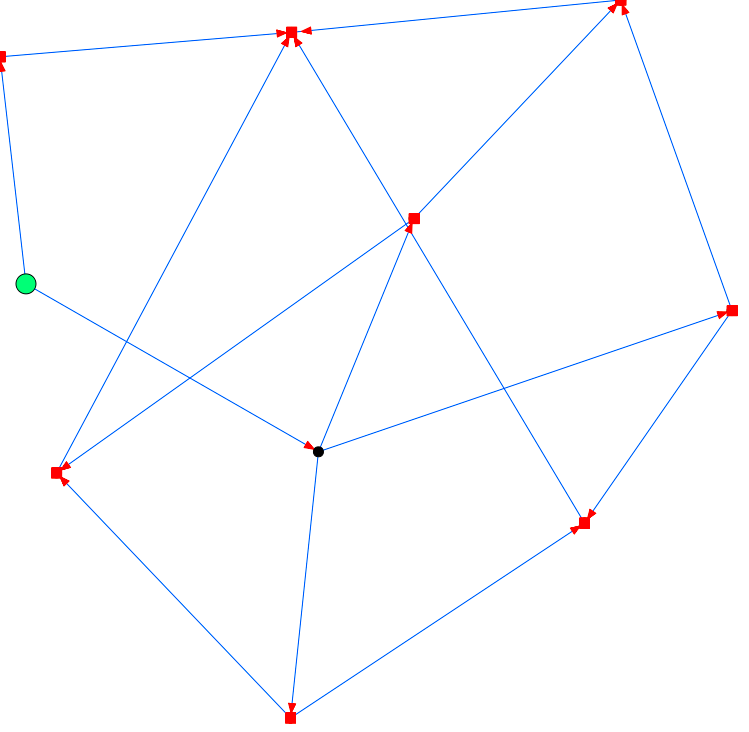
\includegraphics[height=\exampleheight]{../images/SelfRef_2_MAJOR.png}
	\caption
	[$\lambda x.(x x x a) (\lambda x.(x x x) \lambda x.(x x))$]
	{The graph $G_\beta\big(\lambda x.(x x x a) (\lambda x.(x x x) \lambda x.(x x))\big)$
	has eight nodes in which the reduction can ``stay'' -- in the same sense where a 
	DFA can ``stay'' in a certain state through self-referencing. 
	Drawn with the Majorization algorithm.}
	\label{fig:images_SelfRef_1_MAJOR}
\end{figure}

\begin{figure}[htbp]
	% #x.(#y.(y y y y x x y)) #x.(#y.(y y y y x x y)) #x.(x)
	\centering
	\subfigure[Neato produces the graph that one would intuitively draw.]{
		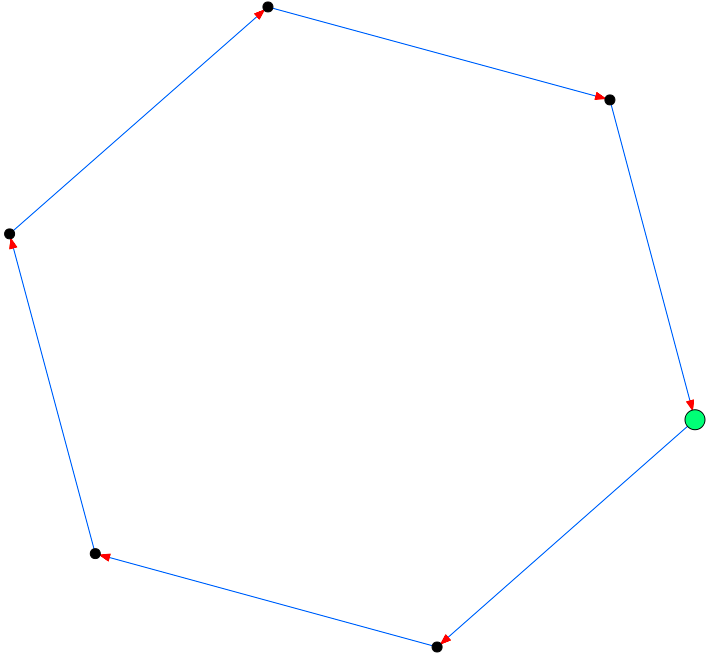
\includegraphics[height=\exampleheight]{../images/Circle_1_NEATO.png}
	}
	\hspace{0.5em}
	\subfigure[The two rightmost nodes are connected, but the Dot algorithm has 
	computed the curve connecting them such that it exceeds the drawing area.]{
		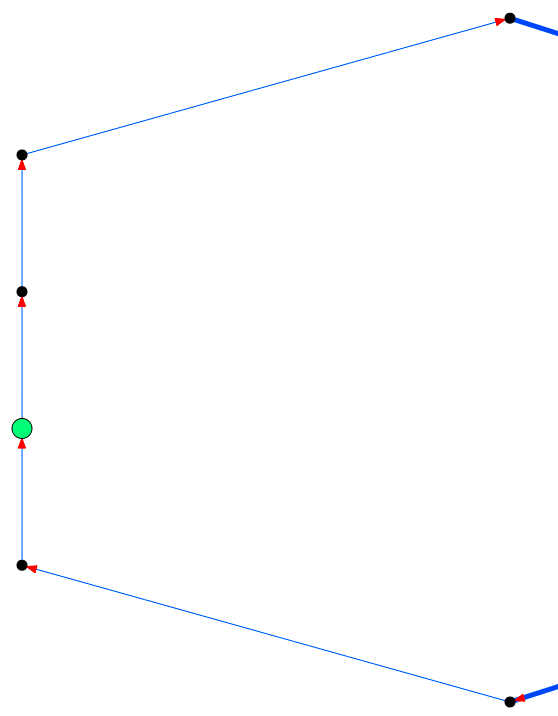
\includegraphics[height=\exampleheight]{../images/Circle_1_DOT.png}
	}
	\hspace{0.5em}
	\subfigure[The Twopi algorithm places all the nodes on a line.]{
		\hspace{2em}
		
\includegraphics[height=\exampleheight]{../images/Circle_1_TWOPI.png}
		\hspace{3em}
	}
	\caption
	[$M M \I$]
	{Some of the algorithms perform poorly on this purely cyclic graph. The
	example term is taken from \cite{VenturiniZilli1984251}. For
	$M\equiv\lambda x.(\lambda y.(y y y y x x y))$ and $\I\equiv\lam{x}{x}$:
	$G_\beta\big(M M \I\big)$.}
	\label{fig:images_Circle_1}
\end{figure}

\begin{figure}[htbp]
	% #x.(#y.(x y y y x x y)) #x.(#y.(y y y y x x y)) #x.(x)
	\centering
	\subfigure[Dot.]{
		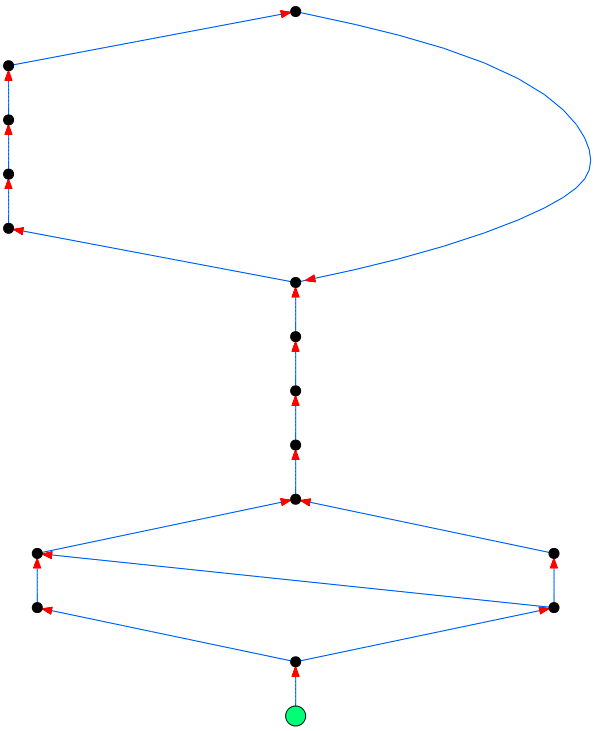
\includegraphics[height=\exampleheight]{../images/Circle_2_DOT.png}
	}
	\subfigure[Circo.]{
		\includegraphics[height=\exampleheight]{../images/Circle_2_CIRCO.png}
	}
	\subfigure[Neato.]{
		\includegraphics[height=\exampleheight]{../images/Circle_2_NEATO.png}
	}
	\subfigure[The Twopi algorithm produces the error from Figure \ref{fig:images_Circle_1}
	on this graph as well. The highlighted edge makes the cycle noticeable.]{
		\includegraphics[height=\exampleheight]{../images/Circle_2_TWOPI.png}
	}
	\caption
	[$\lambda x.(\lambda y.(x y y y x x y)) M \I$]
	{A slightly modified version of the lambda term from Figure \ref{fig:images_Circle_1}
	produces a graph with a that turns cyclic after a few reductions. 
	$G_\beta\big(\lambda x.(\lambda y.(x y y y x x y)) M \I\big)$}
	\label{fig:images_Circle_2}
\end{figure}

\begin{figure}[htbp]
	\centering
	\subfigure[$G_\beta\big(MM\I(MM\I)\big)$ is a prism.]{
		\includegraphics[height=\exampleheight]{../images/Circle_3_NEATO.png}
	}
	\subfigure[$G_\beta\big(MM\I(MM\I)(MM\I)\big)$]{
		\includegraphics[height=\exampleheight]{../images/Circle_4_NEATO.png}
	}
	\subfigure[$G_\beta\big(MM\I(MM\I)(MM\I)(MM\I)\big)$]{
		\includegraphics[height=\exampleheight]{../images/Circle_5_NEATO.png}
	}
	\caption
	[$(MM\I(MM\I)$]
	{If the term from Figure \ref{fig:images_Circle_1} is extended, 
	more complex circular structures occur.}
	\label{fig:images_Circle_35}
\end{figure}

\clearpage

\begin{figure}[htbp]
	\centering
	% #x.(x x x ) #x.(x x x) #x.(x x x ) #x.(x x x)
	\subfigure[$G_\beta\big(\omega_3 \omega_3 \omega_3 \omega_3\big)$]{
		\includegraphics[height=\exampleheight]{../images/Snake_2_NEATO.png}
	}
	% #x.(x x x ) #x.(x x x) (#x.(x x x ) #x.(x x x))
	\subfigure[$G_\beta\big(\omega_3 \omega_3 (\omega_3 \omega_3)\big)$]{
		\includegraphics[height=\exampleheight]{../images/Snake_3_NEATO.png}
	}
	% #x.(x x x ) (#x.(x x x) (#x.(x x x ) #x.(x x x)))
	\subfigure[$G_\beta\big(\omega_3 (\omega_3 (\omega_3 \omega_3))\big)$]{
		\includegraphics[height=\exampleheight]{../images/Snake_4_NEATO.png}
	}

	\caption[$\omega_3 \omega_3 \omega_3 \omega_3$, $\omega_3 \omega_3 (\omega_3 \omega_3)$,
	$\omega_3 (\omega_3 (\omega_3 \omega_3))$]
	{Making terms explicitly right-associative with parentheses
	can drastically affect their reduction graphs. These graphs are
	drawn with the Neato algorithm.}
	\label{fig:images_Snake_2_NEATO}
\end{figure}

\begin{figure}[htbp]
	% #x.(x x) (#x.(x x x) (#x.(x x x) #x.( x x)))
	\centering
	\subfigure[Fdp.]{
		\includegraphics[height=\exampleheight]{../images/SelfRef_1_FDP.png}
	}
	\subfigure[Majorization.]{
		\includegraphics[height=\exampleheight]{../images/SelfRef_1_MAJOR.png}
	}
	\subfigure[Neato.]{
		\includegraphics[height=\exampleheight]{../images/SelfRef_1_NEATO.png}
	}
	\caption[$\omega (\omega_3 (\omega_3 \omega))$]
	{This reduction graph has many nodes in which the reduction can ``stay''.
	The images give an impression of the difference between the three force-directed
	algorithms. $G_\beta\big(\omega (\omega_3 (\omega_3 \omega))\big)$}
	\label{fig:images_SelfRef_1_FDP}
\end{figure}

\begin{figure}[htbp]
	\centering
	\subfigure[$n=1$]{
		\includegraphics[height=1in]{../images/Cube1d_NEATO.png}
	}
	\subfigure[$n=2$]{
		\includegraphics[height=\exampleheight]{../images/Cube2d_NEATO.png}
	}
	\subfigure[$n=3$]{
		\includegraphics[height=\exampleheight]{../images/Cube3d_NEATO.png}
		\label{fig:cube3d}
	}
	\subfigure[$n=4$]{
		\includegraphics[height=\exampleheight]{../images/Cube4d_NEATO.png}
	}
	\subfigure[$n=5$]{
		\includegraphics[height=\exampleheight]{../images/Cube5d_NEATO.png}
	}
	\subfigure[$n=3$, $i2=3$, $i3=2$]{
		\includegraphics[height=\exampleheight]{../images/Cube3d_2_NEATO.png}
	}
	\caption
	[Hypercube.]
	{The reduction graph of the term $((\lam{x_1}{x_1}) f)\hdots((\lam{x_n}{x_n}) f)$,
	$n>0$, where $x_1\hdots x_n$ represent distinct bound variables,
	is an $n$-dimensional hypercube. The graphs are drawn with the Neato algorithm. If
	the term is altered to the more generalized form 
	$((\lam{x_1}{x_1}) f)((\lam{x_2}{x_{2_1} \hdots x_{2_{i2}}}) \lam{y}{y})((\lam{x_3}{x_{3_1} \hdots x_{3_{i3}}}) \lam{y}{y})\hdots((\lam{x_n}{x_{n_1} \hdots x_{n_{in}}}) \lam{y}{y})$,
	the graph produces an $n$-dimensional rectangle with the side lengths
	$i2, i3, \hdots in$.}
	\label{fig:images_Cube1d_NEATO}
\end{figure}

\begin{figure}[htbp]
	\centering
		\includegraphics[height=\exampleheight]{../images/Tetraeder_TWOPI.png}
	\caption
	[Tetrahedron.]
	{This Twopi drawing of the complete graph with four vertices, $K_4$,
	clearly exhibits the fact that it is isomorphic with a tetrahedron. It is
	thus possible to create a lambda term whose reduction graph is the tetrahedron
	as well as a term with the hexahedron as its reduction graph (Figure \ref{fig:cube3d}).
	The term with $K_4$ as its reduction graph is $M_{K_4}\equiv(\lam{x_1}{y}) ((\lam{x_2}{y}) ((\lam{x_3}{y}) (\lam{x_4}{y})))$}
	\label{fig:images_Tetraeder_TWOPI}
\end{figure}


\begin{figure}[htbp]
	\centering
	\subfigure[$n=1$]{
	% #x.(#y.(y x x y)) #x.(#y.(y x x y)) #x.(x)
		\includegraphics[height=\exampleheight]{../images/Polygon3_NEATO.png}
	}
	\subfigure[$n=2$]{
	% #x.(#y.(y y x x y)) #x.(#y.(y y x x y)) #x.(x)
		\includegraphics[height=\exampleheight]{../images/Polygon4_NEATO.png}
	}
	\subfigure[$n=3$]{
	% #x.(#y.(y y y x x y)) #x.(#y.(y y y x x y)) #x.(x)
		\includegraphics[height=\exampleheight]{../images/Polygon5_NEATO.png}
	}
	\subfigure[$n=18$]{
	% #x.(#y.(y y y y y y y y y y y y y y y y y y x x y)) #x.(#y.(y y y y y y y y y y y y y y y y y y x x y)) #x.(x)
		\includegraphics[height=\exampleheight]{../images/Polygon20_NEATO.png}
	}
	\caption
	[Convex, regular polygons.]
	{The graph for the term $\lambda x.(\lambda y.(y_1 \hdots y_n x x y)) \lambda x.(\lambda y.(y_1 \hdots y_n x x y)) \lambda x.(x)$,
	where $n\geq 1$ and $y_1\hdots y_n$ represent repetitions of the variable $y$, 
	produces regular convex polygons with $n+2$ vertices when drawn with Neato. 
	The term $MM\I$ above is a special case of this term. }
	\label{fig:images_Polygon_NEATO}
\end{figure}

\begin{figure}[htbp]
	% #x.(#y.(y y y y y y y x x y)) #x.(#y.(y y y y y y x x y)) #x.(x)
	\centering
	\subfigure[$n=4$, $m=7$]{
		\includegraphics[height=\exampleheight]{../images/Ketcher74_CIRCO.png}
	}
	\subfigure[$n=4$, $m=9$]{
		\includegraphics[height=\exampleheight]{../images/Ketcher94_CIRCO.png}
	}
	\subfigure[$n=6$, $m=9$]{
		\includegraphics[height=\exampleheight]{../images/Ketcher96_CIRCO.png}
	}
	\subfigure[$n=6$, $m=15$]{
		\includegraphics[height=\exampleheight]{../images/Ketcher156_CIRCO.png}
	}
	
	\caption
	[Convex, regular polygons on a string.]
	{If we generalize the term family from Figure \ref{fig:images_Polygon_NEATO} to 
	$\lambda x.(\lambda y.(y_1\hdots y_m x x y)) \lambda x.(\lambda y.(y_1\hdots y_n x x y)) \lambda x.(x)$,
	where $m>n\geq 1$ and $y_1\hdots y_i$ represent repeated usage of the $y$-variable, 
	produces a regular polygon with a ``starting path''. The polygon has $n+2$ vertices
	and the length of the path is $n-m+2$ nodes. The graphs are drawn with Circo.}
	\label{fig:images_Ketcher_CIRCO}
\end{figure}

\begin{figure}[htbp]
	\centering
	\subfigure[$n=3$, $m=2$]{
	% #x.(#y.( y y y x x y)) #x.(#y.( y y y x x y)) #x.(x) (#x.(#y.( y  y)) #x.(#y.( y  y)) #x.(x))
		\includegraphics[height=\exampleheight]{../images/Tube31_NEATO.png}
	}
	\subfigure[$n=6$, $m=5$]{
		\includegraphics[height=\exampleheight]{../images/Tube65_NEATO.png}
	}
	\subfigure[Altering the term to $M_n M_n \I (T T \I)$ where $T\equiv\lam{x}{\lam{y}{x x y}}$ gives
	a tube that seems to continue forever. The tube still consists of $n+2$-sided polygons.]{
	% #x.(#y.(y y y y y y x x y)) #x.(#y.(y y y y y y x x y)) #x.(x) (#x.(#y.(x x y)) #x.(#y.( x x y)) #x.(x))
		\includegraphics[height=\exampleheight]{../images/Tube_long_NEATO.png}
	}
	\caption
	[Tubes.]
	{Let $M_n\equiv\lambda x.(\lambda y.(y_1\hdots y_n x x y))$ and $N_n\equiv\lambda x.(\lambda y.(y_1\hdots y_m))$
	for $n,m\geq 1$, where $y_1\hdots y_i$ denotes the repeating of the variable $y$. 
	The term family $M_n M_n \I (N_m N_m \I)$, where $n,m\geq 1$, produces
	``tubes'' consisting of $m+2$ regular, $n+2$-sided polygons.}
	\label{fig:images_Tube31_NEATO}
\end{figure}

\begin{figure}[htbp]
	\centering
	\renewcommand{\exampleheight}{2.1in}
	\subfigure[$n=3$]{
		\includegraphics[height=\exampleheight]{../images/Regular3_NEATO.png}
	}
	\subfigure[$n=6$]{
	% #x.(#y.(y y y y y y x x y))  #x.(#y.(y y y y y y x x y)) #x.(x) (#x.(#y.(y y y y y y x x y)) #x.(#y.(y y y y y y  x x y)) #x.(x))
		\includegraphics[height=\exampleheight]{../images/Regular6_NEATO.png}
	}
	\subfigure[$n=8$]{
		\includegraphics[height=\exampleheight]{../images/Regular8_NEATO.png}
	}
	\subfigure[$n=12$]{
		\includegraphics[height=\exampleheight]{../images/Regular12_NEATO.png}
	}
	
	\caption
	[Ball-like structures.]
	{Let $M_n\equiv\lambda x.(\lambda y.(y_1\hdots y_n x x y))$ for $n>1$ and
	let $y_1\hdots y_n$ represent the same $y$. The term
	$M_n M_n\I(M_n M_n\I)$, seems to produce a ball-like structure when drawn 
	with Neato. The graph on the title page is the version for $n=15$.}
	\label{fig:images_Regular6_NEATO}
\end{figure}

\begin{figure}[htbp]
	\centering
	% (#x.#y.x (#z.y z y) x) #x.(x) (#x.#y.x (#z.y z y) x)
	\subfigure[Circo.]{
		\includegraphics[height=\exampleheight]{../images/Bohm1_CIRCO.png}
	}
	\subfigure[Dot.]{
		\includegraphics[height=\exampleheight]{../images/Bohm1_DOT.png}
	}
	\subfigure[Neato.]{
		\includegraphics[height=\exampleheight]{../images/Bohm1_NEATO.png}
	}
	\caption
	[$(\lambda x.\lambda y.x (\lambda z.y z y) x) \lambda x.(x) (\lambda x.\lambda y.x (\lambda z.y z y) x)$]
	{The graph $G_\beta\big(H\I H\big)$ where $H\equiv(\lambda x.\lambda y.x (\lambda z.y z y) x)$
	looks a bit like a braid, when drawn with Neato. The term is taken from \cite{Barendregt},
	Exercise 3.5.5(i), and illustrates as such the benefits there are to be gained from
	a tool like this; in \cite{Barendregt}, the task is considered so difficult 
	or tedious that it is worthy of its own Exercise -- with this tool it takes a matter 
	of split seconds to solve it.}
	\label{fig:images_Bohm1_CIRCO}
\end{figure}



% NÆSTEN en fulleren! Bare med valens fire i stedet for valens 3 :(
% #x.(#y.(y y y y y y x x y)) 
% #x.(#y.(y y y y y y x x y)) #x.(x)
% 
% (#x.(#y.(y y y y y y x x y)) 
% #x.(#y.(y y y y y y x x y)) #x.(x)
% )


% #x.(x x) #x.((x x) (x x))
% #x.(#y.(x y) #y.(x y)) #x.(x x) #x.(a)
% #f.(#x.(f (x x))) (#x.(f (x x))) #x.#y.(y (x y))

% ADD: #m.(#n.(#f.(#x.(m f (n f x)))))
% MUL: #m.(#n.(#f.(#x.(m (n f) x))))
% HD: #z.(#p.(p #x.(#y.x)) (#p.(p #x.(#y.y)) z))
% TL: #z.(#p.(p #x.(#y.y)) (#p.(p #x.(#y.y)) z))
% CONS: #x.(#y.(#x.(#y.(#s.(s x y))) #x.(#y.y) (#x.(#y.(#s.(s x y))) x y)))
% EXP: #m.(#n.(#f.(#x.(m n f x))))

% PAIR: #x.(#y.(#s.(s x y)))
% FST: #p.(p #x.(#y.x))
% SND: #p.(p #x.(#y.y))
% TRU: #x.(#y.x)
% FAL:  #x.(#y.y)

% THREE: #f.(#x.(f (f (f x))))
% TWO: #f.(#x.(f (f x)))
% FIVE: #f.(#x.(f (f (f (f (f x))))))
% ZERO: #f.(#x.x)

% succ(succ(succ(ZERO))): #n.(#f.(#x.(f (n f x)))) (#n.(#f.(#x.(f (n f x)))) (#n.(#f.(#x.(f (n f x)))) #f.(#x.x)))

% hd five: #z.(#p.(p #x.(#y.x)) (#p.(p #x.(#y.y)) z)) #f.(#x.(f (f (f (f (f x))))))
% cons 2,3: #x.(#y.(#x.(#y.(#s.(s x y))) #x.(#y.y) (#x.(#y.(#s.(s x y))) x y))) #f.(#x.(f (f x))) #f.(#x.(f (f (f x))))
% cons 3,2: #x.(#y.(#x.(#y.(#s.(s x y))) #x.(#y.y) (#x.(#y.(#s.(s x y))) x y))) #f.(#x.(f (f (f x)))) #f.(#x.(f (f x))) 
% cons 3,3: #x.(#y.(#x.(#y.(#s.(s x y))) #x.(#y.y) (#x.(#y.(#s.(s x y))) x y))) #f.(#x.(f (f (f x)))) #f.(#x.(f (f (f x)))) 
% cons 2,2: #x.(#y.(#x.(#y.(#s.(s x y))) #x.(#y.y) (#x.(#y.(#s.(s x y))) x y))) #f.(#x.(f (f x))) #f.(#x.(f (f x))) 
% cons 5,2: #x.(#y.(#x.(#y.(#s.(s x y))) #x.(#y.y) (#x.(#y.(#s.(s x y))) x y))) #f.(#x.(f (f (f (f (f x)))))) #f.(#x.(f (f x))) 

%lambda L. (hd L + hd tl L)::(F tl L)
% !fib: #L.(#x.(#y.(#x.(#y.(#s.(s x y))) #x.(#y.y) (#x.(#y.(#s.(s x y))) x y))) 
%				(#m.(#n.(#f.(#x.(m f (n f x))))) 
%					(#z.(#p.(p #x.(#y.x)) (#p.(p #x.(#y.y)) z)) L) 
%					(#z.(#p.(p #x.(#y.x)) (#p.(p #x.(#y.y)) z)) #z.(#p.(p #x.(#y.y)) (#p.(p #x.(#y.y)) z)) L))
%				(#f.(#x.(f (f (f (f (f x))))))))

% 2**2: #m.(#n.(#f.(#x.(m n f x)))) #f.(#x.(f (f x))) #f.(#x.(f (f x)))
% 2*2: #m.(#n.(#f.(#x.(m (n f) x)))) #f.(#x.(f (f x))) #f.(#x.(f (f x)))
% 2+2: #m.(#n.(#f.(#x.(m f (n f x))))) #f.(#x.(f (f x))) #f.(#x.(f (f x)))

% 5*5: #m.(#n.(#f.(#x.(m (n f) x)))) #f.(#x.(f (f (f (f (f x)))))) #f.(#x.(f (f (f (f (f x)))))) 
% 5*1: #m.(#n.(#f.(#x.(m (n f) x)))) #f.(#x.(f (f (f (f (f x)))))) #f.(#x.(f x))
% 1*1: #m.(#n.(#f.(#x.(m (n f) x)))) #f.(#x.(f x)) #f.(#x.(f x))
% 2*3: #m.(#n.(#f.(#x.(m (n f) x)))) #f.(#x.(f (f x))) #f.(#x.(f (f (f x))))
% 2+3: #m.(#n.(#f.(#x.(m f (n f x))))) #f.(#x.(f (f x))) #f.(#x.(f (f (f x))))


% IFTHENELSE := #p.(#a.(#b.(p a b)))
% ISZERO :=  #n.(n (#a.(#x.(#y.y))) #x.(#y.x))
% PRED := #n.(#f.(#x.(n (#g.(#h.(h (g f)))) (#u.x) (#u.u))))
% SUB := #m.(#n.(n #n.(#f.(#x.(n (#g.(#h.(h (g f)))) (#u.x) (#u.u)))) m))
% SUCC := #n.(#f.(#x.(f (n f x))))

% succ(succ(5)): #n.(#f.(#x.(f (n f x)))) (#n.(#f.(#x.(f (n f x)))) #f.(#x.(f (f (f (f (f x)))))))

% succ(5): #n.(#f.(#x.(f (n f x)))) #f.(#x.(f (f (f (f (f x))))))
% pred(5): #n.(#f.(#x.(n (#g.(#h.(h (g f)))) (#u.(x)) (#u.(u))))) #f.(#x.(f (f (f (f (f x))))))

% "if V == 0: TWO else THREE"
% #V.(#p.(#a.(#b.(p a b))) (#n.(n (#a.(#x.(#y.y))) #x.(#y.x)) V) #f.(#x.(f (f x))) #f.(#x.(f (f (f x))))) #f.(#x.x)

%g := λr. λn.(1, if n = 0; else n × (r r (n-1)))
%f := g g
% g: #r.(#n.(
%	#p.(#a.(#b.(p a b))) (#n.(n (#a.(#x.(#y.y))) #x.(#y.x)) n)
%	#f.(#x.(f x))
%	(#m.(#n.(#f.(#x.(m (n f) x)))) (r r (#m.(#n.(n #n.(#f.(#x.(n (#g.(#h.(h (g f)))) (#u.x) (#u.u)))) m)) n #f.(#x.(f x)))))))

% fac(2): (#r.(#n.(#p.(#a.(#b.(p a b))) (#n.(n (#a.(#x.(#y.y))) #x.(#y.x)) n) #f.(#x.(f x)) (#m.(#n.(#f.(#x.(m (n f) x)))) (r r (#m.(#n.(n #n.(#f.(#x.(n (#g.(#h.(h (g f)))) (#u.x) (#u.u)))) m)) n #f.(#x.(f x))))))) #r.(#n.(#p.(#a.(#b.(p a b))) (#n.(n (#a.(#x.(#y.y))) #x.(#y.x)) n) #f.(#x.(f x)) (#m.(#n.(#f.(#x.(m (n f) x)))) (r r (#m.(#n.(n #n.(#f.(#x.(n (#g.(#h.(h (g f)))) (#u.x) (#u.u)))) m)) n #f.(#x.(f x)))))))) #f.(#x.(f x))

% PAIR := #x.(#y.(#f.(f x y)))
% FIRST := #p.(p #x.(#y.x))
% SECOND := #p.(p #x.(#y.y))
% NIL := #a.(#x.(#y.x))
% NULL := #p.(p (#x.(#y.(#x.(#y.y)))))
% Φ := #x.(#x.(#y.(#f.(f x y))) (#p.(p #x.(#y.y)) x) (#n.(#f.(#x.(f (n f x)))) (#p.(p #x.(#y.y)) x)))
% PRED := #n.(#p.(p #x.(#y.x)) (n #x.(#x.(#y.(#f.(f x y))) (#p.(p #x.(#y.y)) x) (#n.(#f.(#x.(f (n f x)))) (#p.(p #x.(#y.y)) x))) (#x.(#y.(#f.(f x y))) #f.(#x.x) #f.(#x.x)))) #f.(#x.(f (f x)))

% K := λxy.x
% S := λxyz.(x z (y z))	